% 以下の3行は変更しないこと.
\documentclass[T]{compsoft}
\taikai{2021}
\pagestyle {empty}

\usepackage [dvipdfmx] {graphicx}
\usepackage [dvipdfmx] {color}

% ここに,使用するパッケージを列挙する.
\usepackage{amsthm,amsmath,amssymb}
\usepackage{url}
\usepackage{enumerate,mathdots} % 箇条書き・左下向きの3点リーダー
\usepackage{tikz,here} % 図・コード
\usetikzlibrary{intersections,calc,arrows.meta,positioning}

% ユーザが定義したマクロなどはここに置く.
% ただし学会誌のスタイルの再定義は原則として避けること.
\usepackage{mymacro}
\usepackage{mystyle}

% コマンド一覧
\def\colorF{\textit{color}}
\def\Color{\textit{Color}}
\def\mix{\textit{mix}}
\def\red{\textit{red}}
\def\blu{\textit{blu}}
\def\yel{\textit{yel}}
\def\mix{\textit{mix}}
\def\colorYB{\textit{colorYB}}
\def\colorBYB{\textit{colorBYB}}
\def\colorYBBY{\textit{colorYBBY}}
\def\cposYB{\textit{cposYB}}
\def\cposBYB{\textit{cposBYB}}
\def\cposYBBY{\textit{cposYBBY}}
\def\lift{\textit{liftp}}
\def\cpos{\textit{cpos}}
\def\Cpos{\textit{Cpos}}
\def\WCTF{\textit{Triangle}}
\def\TF{\textit{TriangleF}}
\def\WCT{\textit{WellColoredTriangle}}
\def\WCTF{\textit{WellColoredTriangleF}}
\def\mixCut{\textit{mixCut}}
\def\AllRed{\textit{AllRed}}
\def\falseColor{\textit{falseColor}}
\def\Cexists{\textit{C\_exists}}
\def\Cuniq{\textit{C\_uniq}}
\def\Cmix{\textit{C\_mix}}
\def\Cpaint{\textit{C\_paint}}
\def\Fmix{\textit{Fmix}}
\def\EvenA{\textit{EvenA}}
\def\EvenB{\textit{EvenB}}
\def\Even{\textit{Even}}
\def\ShortOddA{\textit{ShortOddA}}
\def\ShortOddB{\textit{ShortOddB}}
\def\ShortOddC{\textit{ShortOddC}}
\def\ShortOdd{\textit{ShortOdd}}
\def\LongOddA{\textit{LongOddA}}
\def\LongOddB{\textit{LongOddB}}
\def\LongOddC{\textit{LongOddC}}
\def\LongOdd{\textit{LongOdd}}

\begin{document}

% 論文のタイトル
\title{
  Coq による三角形三色問題の証明
}

\author{橋本 翔太 木村 大輔
  %
  % ここにタイトル英訳 (英文の場合は和訳) を書く.
  \ejtitle{
    A formal proof for the three-colored triangle problem on Coq
  }
  %
  % 所属 (和文および英文) を書く.複数著者の所属はまとめてよい.
  \shozoku{Shota Hashimoto}{東邦大学大学院理学研究科}%
  {Toho University}  
  \shozoku{Daisuke Kimura}{東邦大学大学院理学研究科}%
  {Toho University}
  %
  \shutten
  \uketsuke{2099}{99}{99} % dummy
}


\Jabstract{
  Coq とは数学の証明作成を支援する定理証明支援系である.人間は Coq と対話的に証明作成を行うことで誤りを排除した信頼できる証明を得ることができる. 三角形三色問題とは,$n$ 段の逆三角形に配置された六角形のマスに対して,互いに隣接する任意の3マスの色が全て同じかどれも異なるように逆三角形を3色で塗り分けたとき,逆三角形の3頂点のマスの色が必ず全て同じ,もしくはどれも異なるような段数の一般項を求める問題である.この問題は雑誌「数学セミナー」の「エレガントな解答もとむ」欄に出題されており,一般項は $3^k$ 段の形で表せることが示されている.本研究では,数学セミナーでの証明をCoqで形式化して証明を完成させた. これにより,幾何的な直観に頼った側面のあった元の議論を論理に基づいた形式的な証明に直すことができた.
}

\maketitle \thispagestyle {empty}

% 導入
\section{はじめに}
% Coq + ssreflect の説明
Coq~\cite{Coq} とは数学の定理や補題,主張の正しさを保証するためのソフトウェアの$1$つである.
証明の作成中の各場面で示すべき主張(サブゴール)に対して人間がサブゴールを示すための次の一手を指示するとCoqは次のサブゴールを提示し,人間の次の一手を待つ.
このような対話的なやりとりによりCoqは証明の完成の手助けをする.こういったソフトウェアを定理証明支援系と呼ぶ.
証明の規模が大きくなると,複雑な場合分けの漏れがあったり計算ミスなど機械的操作のミスにより人間は誤った証明をしてしまうことがある.
Coq の支援を受けることで,このような誤りが排除された信頼できる証明を得ることができる.
また,Coq はプログラミング言語でもあるため,作成した証明の複製が容易である.
Coq を用いて作成した証明ファイルを公開することで他の人がライブラリとして利用することができる.
既に示された定理は保証済みのものとして,多くの人が各々の目的達成のために利用することができる.
このように,公開された証明1つ1つがたとえ小さな証明であっても組み合わせることで規模の大きな証明の定理を示しやすくなる.

本研究では,Coq + SSReflect を用いて三角形三色問題の証明の形式化を完成させた.
\footnote{
  \url{https://github.com/SyotaHashimoto/ThreeColor}から完成させたCoqのコードをダウンロードすることができる.
}
SSReflect~\cite{SSReflect,CoqBook} は「証明によるリーズニングよりも計算を積極的に用いた方が証明は簡略化される」(ポワンカレ原理)のポリシーに基づいて設計された Coq の拡張ライブラリである.
簡単な同値変形で示すことができる命題論理や等式・不等式に関する主張の証明などは論理式として推論で示すよりもブール型の項と見なして変形した方が効率がよく,SSReflect はその機能を提供する.

三角形三色問題~\cite{Nishiyama1,Nishiyama2,Nishiyama3}とは,次のような問題である:$n$段の逆三角形に配置された正六角形のすべてのマスを異なる3色を用いて色分けをする.ただし,隣り合う2マスとそれらに接する下の段のマスの色は,どれも同じかどれも異なるように塗り分ける.このとき,逆三角形の段数が 3, 9, 27 段の場合 \footnote{本稿では0段目, 1段目, 2段目,$\ldots$と数える.「$n$段の逆三角形」と書いた場合,一辺のマスの個数は$n+1$個である.} は,規則に従ったどのような色の塗り方をしても逆三角形の端点の3マスの色はどれも同じかどれも異なるが,一般にはこのような性質は成り立たない.このような性質を満たす段数の一般項は何か?という問題である.この問題の解決方法は大きく分けて3つの方法が知られている.\cite{Nishiyama1}
\begin{enumerate}
\item \label{ans_1}
  パスカルの三角形の値をmod $3$としたものをマスの色と対応させて使い,代数学での $Lucas$ の定理と関係のある命題を示すことで解決する方法.
\item \label{ans_2}
  逆三角形のマスの塗り方が$n$個の独立パターンに分解できること利用して,重ね合わせの原理を用いることで解決する方法.
\item \label{ans_3}
  比較的少ない段数で成立する段数を調べて段数の規則性(数列)を見つけ出し,この数列から予測できる段数の一般項を推測する方法.
\end{enumerate}
\ref{ans_3}の方法において一般項が$3^k$段であると推測されており,推測された一般項の段数でないならば逆三角形の塗り方の規則に従わない反例が存在することも知られている.

% やったこと
本研究では\ref{ans_3}.の方法で推測して得られた一般項が必要十分条件になっていることを Coq+SSReflect を用いて証明した.
Coq に実装するにあたって,三角形三色問題は幾何的な側面を多くもつ問題であるためこのままでは Coq にコードとして実装することができない.
そこで,三角形のマスの状況を表現する論理式を用意し,色塗り規則を公理化することで三角形三色問題の状況を形式化した.
また,十分条件の証明の方法としては一般項に現れる自然数$k$に関する数学的帰納法を用いて証明した.
一方で,必要条件は対偶法と$n$について場合分けをすることで証明した.

% もくじ
本論文は
第$2$章では三角形三色問題の証明の概要について述べる.
第$3$章では三角形三色問題の証明をCoqに実装するために必要な準備について述べる.
第$4$章では実際にCoqに実装した三角形三色問題の証明について述べる.
第$5$章ではまとめを述べる.

% 三角形三色問題の概要(数学)
% 調和彩色三角形 (well-colored triangle)
% 彩色三角形が調和している
% 彩色三角形が調和性をみたす
\section{三角形三色問題の概要}
三角形三色問題について述べる前に調和性と調和彩色三角形の定義について先に述べる.
以下,$3$色のどれかの色が塗られた同じ大きさの正六角形のマスが平面上に逆三角形の形に敷き詰められている状況を考える (図~\ref{fig:nine_steps}参照)
\footnote{
  ここでは青,赤,黄の三色を用いることにし,各マスにはそれぞれ B, R, Y を記入している.
}.

\begin{dfn}[調和性] \label{dfn:wc}\rm
  (隣接しているとは限らない) $3$つのマスに塗られている色がすべて同じか相異なるとき,
  この$3$マスは{\em 調和性}を満たすという.
\end{dfn}

\begin{exm}
  図$\ref{wellcoloed}$のような$3$マスの組は調和性を満たしているが,
  図$\ref{notwellcoloed}$のような$3$マスの組は調和性を満たしていない.
  \begin{figure}[h]
    \centering
    % wellcolored
\begin{tikzpicture}[scale=0.25]
  % 左図
  \begin{scope}[xshift={-150}]
    \myHexB{-1}{1}
    \myHexY{1}{1}
    \myHexR{0}{0}
  \end{scope}
  % 右図  
  \begin{scope}[xshift={150}]
    \myHexY{-1}{1}
    \myHexY{1}{1}
    \myHexY{0}{0}
  \end{scope}
\end{tikzpicture}

    \caption{調和性を満たす$3$色の組}
    \label{wellcoloed}
  \end{figure}
  \begin{figure}[h]
    \centering
    \definecolor{grayR}{rgb}{0.50, 0.50, 0.50}
\definecolor{grayB}{rgb}{0.10, 0.10, 0.10}
\definecolor{grayY}{rgb}{1.00, 1.00, 1.00}
%\def\myRed{red}
%\def\myBlue{blue}
%\def\myYellow{yellow}
\def\myRed{grayR}
\def\myBlue{grayB}
\def\myYellow{grayY}

% wellcolored

\begin{tikzpicture}[scale=0.25]
  %1段目
  \filldraw[fill=\myRed,xshift={-25*5},yshift={25*sqrt(3)*3}] (0,0)--++(30:1)--++(90:1)--++(150:1)--++(210:1)--++(270:1)--cycle;
  \filldraw[fill=\myYellow,xshift={25*5},yshift={25*sqrt(3)*3}] (0,0)--++(30:1)--++(90:1)--++(150:1)--++(210:1)--++(270:1)--cycle;
  %0段目
  \filldraw[fill=\myBlue,xshift={-25*4},yshift={25*sqrt(3)*4}] (0,0)--++(30:1)--++(90:1)--++(150:1)--++(210:1)--++(270:1)--cycle;
  \filldraw[fill=\myBlue,xshift={-25*6},yshift={25*sqrt(3)*4}] (0,0)--++(30:1)--++(90:1)--++(150:1)--++(210:1)--++(270:1)--cycle;
  \filldraw[fill=\myYellow,xshift={25*6},yshift={25*sqrt(3)*4}] (0,0)--++(30:1)--++(90:1)--++(150:1)--++(210:1)--++(270:1)--cycle;
  \filldraw[fill=\myRed,xshift={25*4},yshift={25*sqrt(3)*4}] (0,0)--++(30:1)--++(90:1)--++(150:1)--++(210:1)--++(270:1)--cycle;
\end{tikzpicture}

    \caption{調和性を満たさない$3$色の組}
    \label{notwellcoloed}
  \end{figure}
\end{exm}

\begin{dfn}[彩色三角形] \label{dfn:three_tri}\rm
  隣接した全ての$3$マスが調和性を満たすように色が塗られた逆三角形を
  {\em 彩色三角形}という.
\end{dfn}

\begin{dfn}[調和彩色三角形] \label{dfn:wc_tri}\rm
  $3$つの端点のマスに塗られている色が調和性を満たしている彩色三角形を{\em 調和彩色三角形} (well-colored triangle) という.
\end{dfn}

次に三角形三色問題について述べる.
  $n(>0)$段の彩色三角形がある.
  図\ref{fig:nine_steps}は$n=9$のときの彩色三角形である.
  このとき,最下段のマスの色は赤であり,最上段の両端のマスは黄,青であるから
  最上段の両端のマスの色と最下段のマスの色について調和性を満たしている (つまり,調和彩色三角形である) ことが分かる.

\begin{figure}[h]
    \centering
    \definecolor{grayR}{rgb}{0.10, 0.10, 0.10}
\definecolor{grayB}{rgb}{0.50, 0.50, 0.50}
\definecolor{grayY}{rgb}{1.00, 1.00, 1.00}
%\def\myRed{red}
%\def\myBlue{blue}
%\def\myYellow{yellow}
\def\myRed{grayR}
\def\myBlue{grayB}
\def\myYellow{grayY}

% 9steps

\begin{tikzpicture}[scale=0.25]
  %9段目
  \filldraw[fill=\myRed] (0,0)--++(30:1)--++(90:1)--++(150:1)--++(210:1)--++(270:1)--cycle;
  %8段目
  \filldraw[fill=\myYellow,xshift={-25},yshift={25*sqrt(3)}] (0,0)--++(30:1)--++(90:1)--++(150:1)--++(210:1)--++(270:1)--cycle;
  \filldraw[fill=\myBlue,xshift={25},yshift={25*sqrt(3)}] (0,0)--++(30:1)--++(90:1)--++(150:1)--++(210:1)--++(270:1)--cycle;
  %7段目
  \filldraw[fill=\myYellow,xshift={-25*2},yshift={25*sqrt(3)*2}] (0,0)--++(30:1)--++(90:1)--++(150:1)--++(210:1)--++(270:1)--cycle;
  \filldraw[fill=\myYellow,yshift={25*sqrt(3)*2}] (0,0)--++(30:1)--++(90:1)--++(150:1)--++(210:1)--++(270:1)--cycle;
  \filldraw[fill=\myRed,xshift={25*2},yshift={25*sqrt(3)*2}] (0,0)--++(30:1)--++(90:1)--++(150:1)--++(210:1)--++(270:1)--cycle;
  %6段目
  \filldraw[fill=\myBlue,xshift={-25*3},yshift={25*sqrt(3)*3}] (0,0)--++(30:1)--++(90:1)--++(150:1)--++(210:1)--++(270:1)--cycle;
  \filldraw[fill=\myRed,xshift={-25},yshift={25*sqrt(3)*3}] (0,0)--++(30:1)--++(90:1)--++(150:1)--++(210:1)--++(270:1)--cycle;
  \filldraw[fill=\myBlue,xshift={25},yshift={25*sqrt(3)*3}] (0,0)--++(30:1)--++(90:1)--++(150:1)--++(210:1)--++(270:1)--cycle;
  \filldraw[fill=\myYellow,xshift={25*3},yshift={25*sqrt(3)*3}] (0,0)--++(30:1)--++(90:1)--++(150:1)--++(210:1)--++(270:1)--cycle;
  %5段目
  \filldraw[fill=\myYellow,xshift={-25*4},yshift={25*sqrt(3)*4}] (0,0)--++(30:1)--++(90:1)--++(150:1)--++(210:1)--++(270:1)--cycle;
  \filldraw[fill=\myRed,xshift={-25*2},yshift={25*sqrt(3)*4}] (0,0)--++(30:1)--++(90:1)--++(150:1)--++(210:1)--++(270:1)--cycle;
  \filldraw[fill=\myRed,yshift={25*sqrt(3)*4}] (0,0)--++(30:1)--++(90:1)--++(150:1)--++(210:1)--++(270:1)--cycle;
  \filldraw[fill=\myYellow,xshift={25*2},yshift={25*sqrt(3)*4}] (0,0)--++(30:1)--++(90:1)--++(150:1)--++(210:1)--++(270:1)--cycle;
  \filldraw[fill=\myYellow,xshift={25*4},yshift={25*sqrt(3)*4}] (0,0)--++(30:1)--++(90:1)--++(150:1)--++(210:1)--++(270:1)--cycle;
  %4段目
  \filldraw[fill=\myRed,xshift={-25*5},yshift={25*sqrt(3)*5}] (0,0)--++(30:1)--++(90:1)--++(150:1)--++(210:1)--++(270:1)--cycle;
  \filldraw[fill=\myBlue,xshift={-25*3},yshift={25*sqrt(3)*5}] (0,0)--++(30:1)--++(90:1)--++(150:1)--++(210:1)--++(270:1)--cycle;
  \filldraw[fill=\myYellow,xshift={-25*1},yshift={25*sqrt(3)*5}] (0,0)--++(30:1)--++(90:1)--++(150:1)--++(210:1)--++(270:1)--cycle;
  \filldraw[fill=\myBlue,xshift={25*1},yshift={25*sqrt(3)*5}] (0,0)--++(30:1)--++(90:1)--++(150:1)--++(210:1)--++(270:1)--cycle;
  \filldraw[fill=\myRed,xshift={25*3},yshift={25*sqrt(3)*5}] (0,0)--++(30:1)--++(90:1)--++(150:1)--++(210:1)--++(270:1)--cycle;
  \filldraw[fill=\myBlue,xshift={25*5},yshift={25*sqrt(3)*5}] (0,0)--++(30:1)--++(90:1)--++(150:1)--++(210:1)--++(270:1)--cycle;
  %3段目
  \filldraw[fill=\myRed,xshift={-25*6},yshift={25*sqrt(3)*6}] (0,0)--++(30:1)--++(90:1)--++(150:1)--++(210:1)--++(270:1)--cycle;
  \filldraw[fill=\myRed,xshift={-25*4},yshift={25*sqrt(3)*6}] (0,0)--++(30:1)--++(90:1)--++(150:1)--++(210:1)--++(270:1)--cycle;
  \filldraw[fill=\myYellow,xshift={-25*2},yshift={25*sqrt(3)*6}] (0,0)--++(30:1)--++(90:1)--++(150:1)--++(210:1)--++(270:1)--cycle;
  \filldraw[fill=\myYellow,yshift={25*sqrt(3)*6}] (0,0)--++(30:1)--++(90:1)--++(150:1)--++(210:1)--++(270:1)--cycle;
  \filldraw[fill=\myRed,xshift={25*2},yshift={25*sqrt(3)*6}] (0,0)--++(30:1)--++(90:1)--++(150:1)--++(210:1)--++(270:1)--cycle;
  \filldraw[fill=\myRed,xshift={25*4},yshift={25*sqrt(3)*6}] (0,0)--++(30:1)--++(90:1)--++(150:1)--++(210:1)--++(270:1)--cycle;
  \filldraw[fill=\myYellow,xshift={25*6},yshift={25*sqrt(3)*6}] (0,0)--++(30:1)--++(90:1)--++(150:1)--++(210:1)--++(270:1)--cycle;
  %2段目
  \filldraw[fill=\myBlue,xshift={-25*7},yshift={25*sqrt(3)*7}] (0,0)--++(30:1)--++(90:1)--++(150:1)--++(210:1)--++(270:1)--cycle;
  \filldraw[fill=\myYellow,xshift={-25*5},yshift={25*sqrt(3)*7}] (0,0)--++(30:1)--++(90:1)--++(150:1)--++(210:1)--++(270:1)--cycle;
  \filldraw[fill=\myBlue,xshift={-25*3},yshift={25*sqrt(3)*7}] (0,0)--++(30:1)--++(90:1)--++(150:1)--++(210:1)--++(270:1)--cycle;
  \filldraw[fill=\myRed,xshift={-25*1},yshift={25*sqrt(3)*7}] (0,0)--++(30:1)--++(90:1)--++(150:1)--++(210:1)--++(270:1)--cycle;
  \filldraw[fill=\myBlue,xshift={25*1},yshift={25*sqrt(3)*7}] (0,0)--++(30:1)--++(90:1)--++(150:1)--++(210:1)--++(270:1)--cycle;
  \filldraw[fill=\myYellow,xshift={25*3},yshift={25*sqrt(3)*7}] (0,0)--++(30:1)--++(90:1)--++(150:1)--++(210:1)--++(270:1)--cycle;
  \filldraw[fill=\myBlue,xshift={25*5},yshift={25*sqrt(3)*7}] (0,0)--++(30:1)--++(90:1)--++(150:1)--++(210:1)--++(270:1)--cycle;
  \filldraw[fill=\myRed,xshift={25*7},yshift={25*sqrt(3)*7}] (0,0)--++(30:1)--++(90:1)--++(150:1)--++(210:1)--++(270:1)--cycle;
  %1段目
  \filldraw[fill=\myRed,xshift={-25*8},yshift={25*sqrt(3)*8}] (0,0)--++(30:1)--++(90:1)--++(150:1)--++(210:1)--++(270:1)--cycle;
  \filldraw[fill=\myYellow,xshift={-25*6},yshift={25*sqrt(3)*8}] (0,0)--++(30:1)--++(90:1)--++(150:1)--++(210:1)--++(270:1)--cycle;
  \filldraw[fill=\myYellow,xshift={-25*4},yshift={25*sqrt(3)*8}] (0,0)--++(30:1)--++(90:1)--++(150:1)--++(210:1)--++(270:1)--cycle;
  \filldraw[fill=\myRed,xshift={-25*2},yshift={25*sqrt(3)*8}] (0,0)--++(30:1)--++(90:1)--++(150:1)--++(210:1)--++(270:1)--cycle;
  \filldraw[fill=\myRed,yshift={25*sqrt(3)*8}] (0,0)--++(30:1)--++(90:1)--++(150:1)--++(210:1)--++(270:1)--cycle;
  \filldraw[fill=\myYellow,xshift={25*2},yshift={25*sqrt(3)*8}] (0,0)--++(30:1)--++(90:1)--++(150:1)--++(210:1)--++(270:1)--cycle;
  \filldraw[fill=\myYellow,xshift={25*4},yshift={25*sqrt(3)*8}] (0,0)--++(30:1)--++(90:1)--++(150:1)--++(210:1)--++(270:1)--cycle;
  \filldraw[fill=\myRed,xshift={25*6},yshift={25*sqrt(3)*8}] (0,0)--++(30:1)--++(90:1)--++(150:1)--++(210:1)--++(270:1)--cycle;
  \filldraw[fill=\myRed,xshift={25*8},yshift={25*sqrt(3)*8}] (0,0)--++(30:1)--++(90:1)--++(150:1)--++(210:1)--++(270:1)--cycle;
  %0段目
  \filldraw[fill=\myYellow,xshift={-25*9},yshift={25*sqrt(3)*9}] (0,0)--++(30:1)--++(90:1)--++(150:1)--++(210:1)--++(270:1)--cycle;
  \filldraw[fill=\myBlue,xshift={-25*7},yshift={25*sqrt(3)*9}] (0,0)--++(30:1)--++(90:1)--++(150:1)--++(210:1)--++(270:1)--cycle;
  \filldraw[fill=\myRed,xshift={-25*5},yshift={25*sqrt(3)*9}] (0,0)--++(30:1)--++(90:1)--++(150:1)--++(210:1)--++(270:1)--cycle;
  \filldraw[fill=\myBlue,xshift={-25*3},yshift={25*sqrt(3)*9}] (0,0)--++(30:1)--++(90:1)--++(150:1)--++(210:1)--++(270:1)--cycle;
  \filldraw[fill=\myYellow,xshift={-25*1},yshift={25*sqrt(3)*9}] (0,0)--++(30:1)--++(90:1)--++(150:1)--++(210:1)--++(270:1)--cycle;
  \filldraw[fill=\myBlue,xshift={25*1},yshift={25*sqrt(3)*9}] (0,0)--++(30:1)--++(90:1)--++(150:1)--++(210:1)--++(270:1)--cycle;
  \filldraw[fill=\myRed,xshift={25*3},yshift={25*sqrt(3)*9}] (0,0)--++(30:1)--++(90:1)--++(150:1)--++(210:1)--++(270:1)--cycle;
  \filldraw[fill=\myBlue,xshift={25*5},yshift={25*sqrt(3)*9}] (0,0)--++(30:1)--++(90:1)--++(150:1)--++(210:1)--++(270:1)--cycle;
  \filldraw[fill=\myYellow,xshift={25*7},yshift={25*sqrt(3)*9}] (0,0)--++(30:1)--++(90:1)--++(150:1)--++(210:1)--++(270:1)--cycle;
  \filldraw[fill=\myBlue,xshift={25*9},yshift={25*sqrt(3)*9}] (0,0)--++(30:1)--++(90:1)--++(150:1)--++(210:1)--++(270:1)--cycle;
\end{tikzpicture}

    \caption{彩色三角形($n=9$のとき)}
    \label{fig:nine_steps}
\end{figure}

$n=9$の場合は最上段の塗り方が図\ref{fig:nine_steps}の塗り方でなくとも逆三角形の$3$つの頂点のマスは調和性を満たすことが観察できる.
このことから次のような仮説が考えられる.
\begin{itemize}
  \item[(仮説)]
  最上段をどのように塗っても最上段の両端のマスの色と最下段のマスの色は調和性を満たす.
\end{itemize}

数学セミナー誌で出題された三角形三色問題は次の$2$つの問題のことである~\cite{Nishiyama2}.
\begin{enumerate}
\item \label{que:1}
  $n=9$のとき仮説が成立することを証明せよ.
\item \label{que:2}
  $n=9$以外に仮説が成立する段数が存在するか調べ,存在するならば$n$の一般式を求めよ.
\end{enumerate}

この問題については既に解答が得られており,
一般に$n=3^k$段の逆三角形において仮説が成立することを示す次の定理\ref{thm:tri_iff}が示されている.

\begin{thm} \label{thm:tri_iff}
  $n(>0)$段の逆三角形に配置されたマス対して,
  最上段のマスを$3$色で任意に塗ったとき
  \[
  (\exists k\in\N.n=3^k) \Leftrightarrow \text{$n$段の逆三角形は常に調和彩色三角形}.
  \]
\end{thm}

本節ではこの定理の証明を Coq で実装するにあたり,証明の概要について述べる.

% 2.1 n=3^k => 調和三角形
\subsection{十分条件}
定理\ref{thm:tri_iff}を証明するにあたって,十分条件と必要条件に分けて話を進める.
ここでは定理\ref{thm:tri_iff}の十分条件である定理\ref{thm:tri_suf}の証明の概要について述べる.
\begin{thm}[十分条件] \label{thm:tri_suf}
  $n$段の逆三角形に配置されたマス対して,
  \[
  (\exists k\in\N.n=3^k) \Imp \text{$n$段の逆三角形は常に調和彩色三角形}.
  \]
\end{thm}
定理\ref{thm:tri_suf}を証明するためには論理同値である次の命題を証明すればよい.
\[
\forall k\in\N.(n=3^k \Imp \text{$n$段の逆三角形は常に調和彩色三角形}).
\]
これは$k$に関する数学的帰納法を用いて証明する.
\begin{itemize}
\item
  $k=0$のときは$n=1$となり明らかに成立する.
\item
  $k$ のとき成立すると仮定する.
  すなわち,$3^{k}$段の逆三角形ならば常に調和彩色三角形であると仮定する.
  
  ここからは図\ref{fig:ind_steps}を用いて証明を進める.
  以下,左から$x$番目,上から$y$段目のマスを$\V{x}{y}$と書くことにし,
  このマスに塗られている色を$\C{x}{y}$とする.  
\begin{figure}[h]
    \centering
    % 3^{k+1} 段の三角形
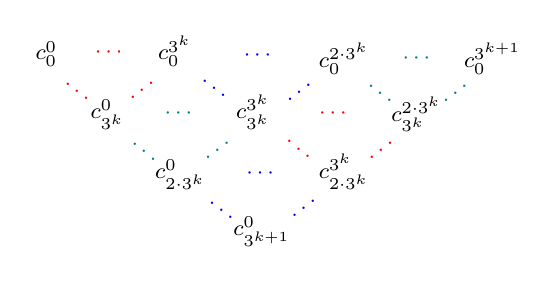
\begin{tikzpicture}
  {\footnotesize{
      % 3^(k+1)段目
      \node (a0) {$c^{0}_{3^{k+1}}$};
      % 2*3^k段目
      \node[above left=0.2cm of a0] (b0) {$c^{0}_{2\cdot3^{k}}$};
      \node[above right=0.2cm of a0] (b1) {$c^{3^{k}}_{2\cdot3^{k}}$};
      % 3^k段目
      \node[above left=0.25cm of b0] (c0) {$c^{0}_{3^{k}}$};
      \node[above right=0.25cm of b0] (c1) {$c^{3^{k}}_{3^{k}}$};
      \node[above right=0.1cm of b1] (c2) {$c^{2\cdot3^{k}}_{3^{k}}$};
      % 0段目
      \node[above left=0.3cm of c0] (d0) {$c^{0}_{0}$};
      \node[above right=0.3cm of c0] (d1) {$c^{3^{k}}_{0}$};
      \node[above left=0.1cm of c2] (d2) {$c^{2\cdot3^{k}}_{0}$};
      \node[above right=0.1cm of c2] (d3) {$c^{3^{k+1}}_{0}$};
      % 点線 [3^(k+1)段 〜 2*3^k 段]
      \node[blue] at ($(a0)!.5!(b0)$) {$\ddots$};
      \node[blue] at ($(b0)!.5!(b1)$) {$\cdots$};
      \node[blue] at ($(a0)!.5!(b1)$) {$\iddots$};
      % 点線 [2*3^k 段 〜 3^k 段]
      \node[teal] at ($(b0)!.5!(c0)$) {$\ddots$};
      \node[teal] at ($(c0)!.5!(c1)$) {$\cdots$};
      \node[teal] at ($(b0)!.5!(c1)$) {$\iddots$};
      \node[red] at ($(b1)!.5!(c1)$) {$\ddots$};
      \node[red] at ($(c1)!.5!(c2)$) {$\cdots$};
      \node[red] at ($(b1)!.5!(c2)$) {$\iddots$};
      % 点線 [3^k 段 〜 0 段]
      \node[red] at ($(c0)!.5!(d0)$) {$\ddots$};
      \node[red] at ($(d0)!.5!(d1)$) {$\cdots$};
      \node[red] at ($(c0)!.5!(d1)$) {$\iddots$};
      \node[blue] at ($(c1)!.5!(d1)$) {$\ddots$};
      \node[blue] at ($(d1)!.5!(d2)$) {$\cdots$};
      \node[blue] at ($(c1)!.5!(d2)$) {$\iddots$};
      \node[teal] at ($(c2)!.5!(d2)$) {$\ddots$};
      \node[teal] at ($(d2)!.5!(d3)$) {$\cdots$};
      \node[teal] at ($(c2)!.5!(d3)$) {$\iddots$};
  }}
\end{tikzpicture}

    \caption{彩色三角形($n=3^{k+1}$のとき)}
    \label{fig:ind_steps}
\end{figure}
ここで,図\ref{fig:ind_steps}の中にあるいくつかの$3^k$段の彩色三角形に注目する.
説明を簡単にするために,頂点$\V{x_0}{y_0}$,$\V{x_1}{y_1}$,$\V{x_2}{y_2}$の彩色三角形を
その$3$つの頂点のマスの色を組にして$(\C{x_0}{y_0},\C{x_1}{y_1},\C{x_2}{y_2})$と表すことにする.
上から$0$段目から$3^{k}$段目の間では次の$3$つの彩色三角形
\begin{center}
$\left(\C{0}{0},\C{3^{k}}{0},\C{0}{3^{k}}\right)$,
\quad
$\left(\C{3^{k}}{0},\C{2\cdot3^{k}}{0},\C{3^{k}}{3^{k}}\right)$,
\\
$\left(\C{2\cdot3^{k}}{0},\C{3^{k+1}}{0},\C{2\cdot3^{k}}{3^{k}}\right)$
\end{center}
に注目すると帰納法の仮定よりこれらは調和彩色三角形である.
よって最上段の$4$つのマスの色$\C{0}{0}$,$\C{3^k}{0}$,$\C{2\cdot 3^k}{0}$,$\C{3^{k+1}}{0}$から
$3^k$段目のマスの色$\C{0}{3^k}$,$\C{3^k}{3^k}$,$\C{2\cdot 3^k}{3^k}$を計算して求めることができる.
また,上から$3^{k}$段目から$2\cdot3^{k}$段目の間にある$2$個の彩色三角形
\[
\left(\C{0}{3^{k}},\C{3^{k}}{3^{k}},\C{0}{2\cdot3^{k}}\right),
\quad
\left(\C{3^{k}}{3^{k}},\C{2\cdot3^{k}}{3^{k}},\C{3^{k}}{2\cdot3^{k}}\right)
\]
も調和彩色三角形 (帰納法の仮定) である.よって$\C{0}{3^k}$,$\C{3^k}{3^k}$,$\C{2\cdot 3^k}{3^k}$から
$2\cdot 3^k$段のマスの色$\C{0}{2\cdot 3^k}$と$\C{3^k}{2\cdot 3^k}$を計算して求めることができる.
同じく帰納法の仮定より,上から$2\cdot3^{k}$段目から$3^{k+1}$段目の間にある彩色三角形
\[
\left(\C{0}{2\cdot3^{k}},\C{3^{k}}{2\cdot3^{k}},\C{0}{3^{k+1}}\right)
\]
も調和彩色三角形である.よって$\C{0}{2\cdot 3^k}$と$\C{3^k}{2\cdot 3^k}$から最下段のマスの色$\C{0}{3^{k+1}}$を得ることができる.
さらに,簡単な計算\footnote{81通りの場合分けをする}により$\C{0}{0}$および$\C{3^{k+1}}{0}$と最下段の色$\C{0}{3^{k+1}}$は調和性を満たすことがいえるので
$(\C{0}{0},\C{3^{k+1}}{0},\C{0}{3^{k+1}})$は調和彩色三角形である.
%これらの$6$個の$3^k$段の彩色三角形はすべて帰納法の仮定より常に調和彩色三角形である.
%よって,調和彩色三角形の定義より最上段のマスの$4$色$c^0_0$,$c^{3^{k}}_0$,$c^{2\cdot3^{k}}_0$,$c^{3^{k+1}}_0$から最下段のマスの$c^0_{3^{k+1}}$の色が得られる.
%% ---------- 未修正 ----------
%最後に,$4$色$c^0_0$,$c^{3^{k}}_0$,$c^{2\cdot3^{k}}_0$,$c^{3^{k+1}}_0$に対して,
%から得られた色は$c^0_0, c^{3^{k+1}}_0$が規則に従った色と等しくなることを
%利用すると,
%% ------------------------------
%最上段の両端のマスに塗られている$2$色$\C{0}{0}$,$\C{3^{k+1}}{0}$と最下段の色$\C{0}{3^{k+1}}$は調和性を満たす.
以上より,$3^{k+1}$段の逆三角形は常に調和彩色三角形である.
\end{itemize}
% 2.2 調和 (well-colored) => n=3^k
\subsection{必要条件}
次は定理\ref{thm:tri_iff}の必要条件である定理\ref{thm:tri_nec}の証明の概要について述べる.
\begin{thm}[必要条件] \label{thm:tri_nec}
  $n(>0)$段の逆三角形に配置されたマス対して,
  \[
  \text{$n$段の逆三角形は常に調和彩色三角形} \Imp (\exists k.n=3^k).
  \]
\end{thm}
定理\ref{thm:tri_nec}の証明では対偶法を用いた後に,$n$に関する場合分けをして証明する.
定理\ref{thm:tri_nec}の対偶は以下の通り.

$\lnot$ $(\exists$ $k\in\N.n=3^k)$ $\Imp$ $\lnot($ $n$段の逆三角形は常に調和彩色三角形$)$.

したがって,$\lnot(\exists k\in\N.n=3^k)$を仮定したとき,次の各場合について調和彩色三角形にならない最上段のマスの塗り方を挙げればよい.
場合分けの仕方は次の$3$つである.
\begin{enumerate}
\item \label{case:even}
  $n$が偶数
\item \label{case:shortodd}
  $n$が奇数 かつ $3^{k} < n \leq 2 \cdot 3^{k}$
\item \label{case:longodd}
  $n$が奇数 かつ $2 \cdot 3^{k} + 1 \leq n < 3^{k+1}$
\end{enumerate}
各場合について調和彩色三角形にならないような最上段のマスの塗り方は次の通り.
\begin{itemize}
  \item
    \ref{case:even}.のときは最上段のマスを黄,青の順で交互に塗る(図~\ref{fig:even_steps}参照).
    すると,$n$が偶数であるため最上段のマス数は奇数個となるから,
    最上段の両端のマスは黄色になり,
    第$1$段目のマスは規則よりすべて赤色で塗られる.
    さらに,もう一方の規則より最下段のマスまですべて赤で塗られている.
    したがって,$n$が偶数であるから最上段の両端のマスは黄であり,最下段のマスの色が赤であるから調和性を満たさないので調和彩色三角形でない.
    \begin{figure}[h]
      \centering
      \definecolor{grayR}{rgb}{0.50, 0.50, 0.50}
\definecolor{grayB}{rgb}{0.10, 0.10, 0.10}
\definecolor{grayY}{rgb}{1.00, 1.00, 1.00}
%\def\myRed{red}
%\def\myBlue{blue}
%\def\myYellow{yellow}
\def\myRed{grayR}
\def\myBlue{grayB}
\def\myYellow{grayY}

% even_steps
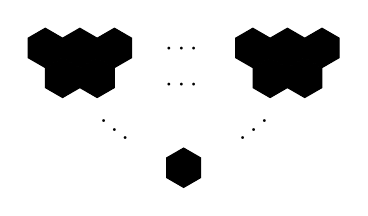
\begin{tikzpicture}[scale=0.25]
  %3^(k'+1)段目
  \filldraw[fill=\myRed,yshift={25*sqrt(3)*3}] (0,0)--++(30:1)--++(90:1)--++(150:1)--++(210:1)--++(270:1)--cycle;
  %2 〜 3^(K'+1)-1段目
  \node[xshift={-25*1},yshift={25*sqrt(3)*1.3}](0,0){$\ddots$};
  \node[xshift={25*1},yshift={25*sqrt(3)*1.3}](0,0){$\iddots$};
  %1段目
  \filldraw[fill=\myRed,xshift={-25*7},yshift={25*sqrt(3)*6}] (0,0)--++(30:1)--++(90:1)--++(150:1)--++(210:1)--++(270:1)--cycle;
  \filldraw[fill=\myRed,xshift={-25*5},yshift={25*sqrt(3)*6}] (0,0)--++(30:1)--++(90:1)--++(150:1)--++(210:1)--++(270:1)--cycle;
  \node[yshift={25*sqrt(3)*1.6}](0,0){$\cdots$};
  \filldraw[fill=\myRed,xshift={25*5},yshift={25*sqrt(3)*6}] (0,0)--++(30:1)--++(90:1)--++(150:1)--++(210:1)--++(270:1)--cycle;
  \filldraw[fill=\myRed,xshift={25*7},yshift={25*sqrt(3)*6}] (0,0)--++(30:1)--++(90:1)--++(150:1)--++(210:1)--++(270:1)--cycle;
  %0段目
  \filldraw[fill=\myYellow,xshift={-25*8},yshift={25*sqrt(3)*7}] (0,0)--++(30:1)--++(90:1)--++(150:1)--++(210:1)--++(270:1)--cycle;
  \filldraw[fill=\myBlue,xshift={-25*6},yshift={25*sqrt(3)*7}] (0,0)--++(30:1)--++(90:1)--++(150:1)--++(210:1)--++(270:1)--cycle;
  \filldraw[fill=\myYellow,xshift={-25*4},yshift={25*sqrt(3)*7}] (0,0)--++(30:1)--++(90:1)--++(150:1)--++(210:1)--++(270:1)--cycle;
  \node[yshift={25*sqrt(3)*1.9}](0,0){$\cdots$};
  \filldraw[fill=\myYellow,xshift={25*4},yshift={25*sqrt(3)*7}] (0,0)--++(30:1)--++(90:1)--++(150:1)--++(210:1)--++(270:1)--cycle;
  \filldraw[fill=\myBlue,xshift={25*6},yshift={25*sqrt(3)*7}] (0,0)--++(30:1)--++(90:1)--++(150:1)--++(210:1)--++(270:1)--cycle;
  \filldraw[fill=\myYellow,xshift={25*8},yshift={25*sqrt(3)*7}] (0,0)--++(30:1)--++(90:1)--++(150:1)--++(210:1)--++(270:1)--cycle;
\end{tikzpicture}

      \caption{$n$が偶数}
      \label{fig:even_steps}
    \end{figure}
  \item
    \ref{case:shortodd}.のときは最上段のマスを外側の両端のマスから内側の方に向かって黄,青の順で$2$色を用いて対称的に交互に塗る(図~\ref{fig:shortodd_steps}参照).
    %% ---------- 未修正 ----------
    すると,補題\ref{lem:tri_suf}より$3^k$段の逆三角形は調和彩色三角形なので,最上段から$3^k$段下のマスは黄,青の順で交互に塗られている.
    これは\ref{case:even}.の場合に帰着できるので最下段のマスの色は赤である.
    したがって,最上段の両端のマスの色は黄であり,最下段のマスの色が赤であるから調和性を満たさないので調和彩色三角形でない.
    %% ------------------------------
    \begin{figure}[h]
      \centering
      % oddshort_steps
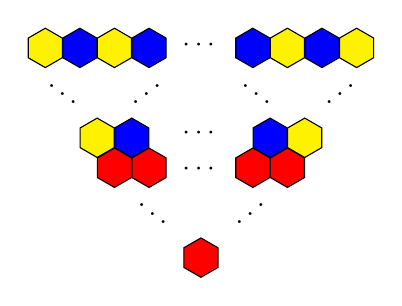
\begin{tikzpicture}[scale=0.25]
  %3^(k'+1)段目
  \filldraw[fill=red,yshift={25*sqrt(3)*2}] (0,0)--++(30:1)--++(90:1)--++(150:1)--++(210:1)--++(270:1)--cycle;
  %3^k'+2 〜 3^(k'+1)-1段目
  \node[yshift={25*sqrt(3)*1.4}](0,0){$\cdots$};
  \node[xshift={-25*0.7},yshift={25*sqrt(3)*1.1}](0,0){$\ddots$};
  \node[xshift={25*0.7},yshift={25*sqrt(3)*1.1}](0,0){$\iddots$};
  %3^k'+1段目
  \filldraw[fill=red,xshift={-25*5},yshift={25*sqrt(3)*5}] (0,0)--++(30:1)--++(90:1)--++(150:1)--++(210:1)--++(270:1)--cycle;
  \filldraw[fill=red,xshift={-25*3},yshift={25*sqrt(3)*5}] (0,0)--++(30:1)--++(90:1)--++(150:1)--++(210:1)--++(270:1)--cycle;
  \node[yshift={25*sqrt(3)*1.7}](0,0){$\cdots$};
  \filldraw[fill=red,xshift={25*3},yshift={25*sqrt(3)*5}] (0,0)--++(30:1)--++(90:1)--++(150:1)--++(210:1)--++(270:1)--cycle;
  \filldraw[fill=red,xshift={25*5},yshift={25*sqrt(3)*5}] (0,0)--++(30:1)--++(90:1)--++(150:1)--++(210:1)--++(270:1)--cycle;
  %3^k'段目
  \filldraw[fill=yellow,xshift={-25*6},yshift={25*sqrt(3)*6}] (0,0)--++(30:1)--++(90:1)--++(150:1)--++(210:1)--++(270:1)--cycle;
  \filldraw[fill=blue,xshift={-25*4},yshift={25*sqrt(3)*6}] (0,0)--++(30:1)--++(90:1)--++(150:1)--++(210:1)--++(270:1)--cycle;
  \filldraw[fill=blue,xshift={25*4},yshift={25*sqrt(3)*6}] (0,0)--++(30:1)--++(90:1)--++(150:1)--++(210:1)--++(270:1)--cycle;
  \filldraw[fill=yellow,xshift={25*6},yshift={25*sqrt(3)*6}] (0,0)--++(30:1)--++(90:1)--++(150:1)--++(210:1)--++(270:1)--cycle;
  %1 〜 3^k'-1段目
  \node[xshift={-25*2},yshift={25*sqrt(3)*2.1}](0,0){$\ddots$};
  \node[xshift={-25*0.8},yshift={25*sqrt(3)*2.1}](0,0){$\iddots$};
  \node[xshift={25*0.8},yshift={25*sqrt(3)*2.1}](0,0){$\ddots$};
  \node[xshift={25*2},yshift={25*sqrt(3)*2.1}](0,0){$\iddots$};
  %0段目
  \filldraw[fill=yellow,xshift={-25*9},yshift={25*sqrt(3)*9}] (0,0)--++(30:1)--++(90:1)--++(150:1)--++(210:1)--++(270:1)--cycle;
  \filldraw[fill=blue,xshift={-25*7},yshift={25*sqrt(3)*9}] (0,0)--++(30:1)--++(90:1)--++(150:1)--++(210:1)--++(270:1)--cycle;
  \filldraw[fill=yellow,xshift={-25*5},yshift={25*sqrt(3)*9}] (0,0)--++(30:1)--++(90:1)--++(150:1)--++(210:1)--++(270:1)--cycle;
  \filldraw[fill=blue,xshift={-25*3},yshift={25*sqrt(3)*9}] (0,0)--++(30:1)--++(90:1)--++(150:1)--++(210:1)--++(270:1)--cycle;
  \node[yshift={25*sqrt(3)*2.3},above=0.01cm](0,0){$\cdots$};
  \filldraw[fill=blue,xshift={25*3},yshift={25*sqrt(3)*9}] (0,0)--++(30:1)--++(90:1)--++(150:1)--++(210:1)--++(270:1)--cycle;
  \filldraw[fill=yellow,xshift={25*5},yshift={25*sqrt(3)*9}] (0,0)--++(30:1)--++(90:1)--++(150:1)--++(210:1)--++(270:1)--cycle;
  \filldraw[fill=blue,xshift={25*7},yshift={25*sqrt(3)*9}] (0,0)--++(30:1)--++(90:1)--++(150:1)--++(210:1)--++(270:1)--cycle;
  \filldraw[fill=yellow,xshift={25*9},yshift={25*sqrt(3)*9}] (0,0)--++(30:1)--++(90:1)--++(150:1)--++(210:1)--++(270:1)--cycle;
\end{tikzpicture}

      \caption{$n$が奇数 かつ $3^{k} < n \leq 2 \cdot 3^{k}$}
      \label{fig:shortodd_steps}
    \end{figure}
  \item
    \ref{case:longodd}.のときは最上段のマスを両端のマスからそれぞれ$3^k$マス内側の方に向かって黄,その他の内側のマスを青を用いて対称的に塗る(図~\ref{fig:longodd_steps}参照).
    このとき,黄で塗られている内側のマスは$n-2\cdot3^k+1$マスである.
    %% ---------- 未修正 ----------
    すると,補題\ref{lem:tri_suf}より$3^k$段の逆三角形は調和彩色三角形なので,最上段から$3^k$段において外側から$n-2\cdot3^k+1$マスはすべて赤で塗られている.
    同様にして,$2\cdot3^k$段下のマスの色はすべて赤で塗られている.
    したがって,最上段の両端のマスの色は黄であり,最下段のマスの色が赤であるから調和性を満たさないので調和彩色三角形でない.
    %% ------------------------------
    \begin{figure}[h]
      \centering
      % oddshort_steps
\definecolor{grayR}{rgb}{0.50, 0.50, 0.50}
\definecolor{grayB}{rgb}{0.10, 0.10, 0.10}
\definecolor{grayY}{rgb}{1.00, 1.00, 1.00}
%\def\myRed{red}
%\def\myBlue{blue}
%\def\myYellow{yellow}
\def\myRed{grayR}
\def\myBlue{grayB}
\def\myYellow{grayY}

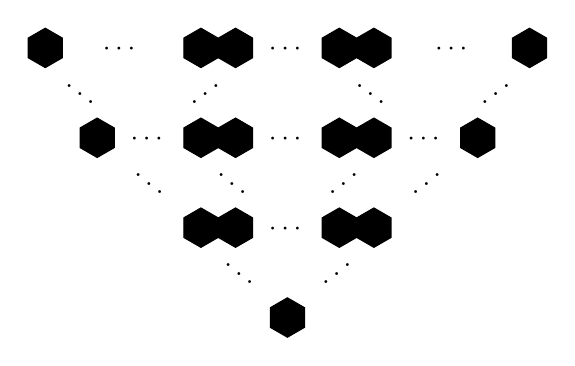
\begin{tikzpicture}[scale=0.25]
  %3^(k'+1)段目
  \filldraw[fill=\myRed,yshift={25*sqrt(3)*5}] (0,0)--++(30:1)--++(90:1)--++(150:1)--++(210:1)--++(270:1)--cycle;
  %3^k'+2 〜 3^(k'+1)-1段目
  \node[xshift={-25*0.7},yshift={25*sqrt(3)*1.85}](0,0){$\ddots$};
  \node[xshift={25*0.7},yshift={25*sqrt(3)*1.85}](0,0){$\iddots$};
  %3^k'+1段目
  \filldraw[fill=\myRed,xshift={-25*5},yshift={25*sqrt(3)*8}] (0,0)--++(30:1)--++(90:1)--++(150:1)--++(210:1)--++(270:1)--cycle;
  \filldraw[fill=\myRed,xshift={-25*3},yshift={25*sqrt(3)*8}] (0,0)--++(30:1)--++(90:1)--++(150:1)--++(210:1)--++(270:1)--cycle;
  \node[yshift={25*sqrt(3)*2.15}](0,0){$\cdots$};
  \filldraw[fill=\myRed,xshift={25*3},yshift={25*sqrt(3)*8}] (0,0)--++(30:1)--++(90:1)--++(150:1)--++(210:1)--++(270:1)--cycle;
  \filldraw[fill=\myRed,xshift={25*5},yshift={25*sqrt(3)*8}] (0,0)--++(30:1)--++(90:1)--++(150:1)--++(210:1)--++(270:1)--cycle;
  %3^k'+1 〜 3^(k'+1)-1段目
  \node[xshift={-25*2},yshift={25*sqrt(3)*2.6}](0,0){$\ddots$};
  \node[xshift={25*0.8},yshift={25*sqrt(3)*2.6}](0,0){$\iddots$};
  \node[xshift={-25*0.8},yshift={25*sqrt(3)*2.6}](0,0){$\ddots$};
  \node[xshift={25*2},yshift={25*sqrt(3)*2.6}](0,0){$\iddots$};
  %3^k'段目
  \filldraw[fill=\myRed,xshift={-25*11},yshift={25*sqrt(3)*11}] (0,0)--++(30:1)--++(90:1)--++(150:1)--++(210:1)--++(270:1)--cycle;
  \node[xshift={-25*2},yshift={25*sqrt(3)*2.9}](0,0){$\cdots$};
  \filldraw[fill=\myRed,xshift={-25*5},yshift={25*sqrt(3)*11}] (0,0)--++(30:1)--++(90:1)--++(150:1)--++(210:1)--++(270:1)--cycle;
  \filldraw[fill=\myYellow,xshift={-25*3},yshift={25*sqrt(3)*11}] (0,0)--++(30:1)--++(90:1)--++(150:1)--++(210:1)--++(270:1)--cycle;
  \node[yshift={25*sqrt(3)*2.9}](0,0){$\cdots$};
  \filldraw[fill=\myYellow,xshift={25*3},yshift={25*sqrt(3)*11}] (0,0)--++(30:1)--++(90:1)--++(150:1)--++(210:1)--++(270:1)--cycle;
  \filldraw[fill=\myRed,xshift={25*5},yshift={25*sqrt(3)*11}] (0,0)--++(30:1)--++(90:1)--++(150:1)--++(210:1)--++(270:1)--cycle;
  \node[xshift={25*2},yshift={25*sqrt(3)*2.9}](0,0){$\cdots$};
  \filldraw[fill=\myRed,xshift={25*11},yshift={25*sqrt(3)*11}] (0,0)--++(30:1)--++(90:1)--++(150:1)--++(210:1)--++(270:1)--cycle;
  %1 〜 3^k'-1段目
  \node[xshift={-25*3},yshift={25*sqrt(3)*3.35}](0,0){$\ddots$};
  \node[xshift={-25*1.2},yshift={25*sqrt(3)*3.35}](0,0){$\iddots$};
  \node[xshift={25*1.2},yshift={25*sqrt(3)*3.35}](0,0){$\ddots$};
  \node[xshift={25*3},yshift={25*sqrt(3)*3.35}](0,0){$\iddots$};
  %0段目
  \filldraw[fill=\myYellow,xshift={-25*14},yshift={25*sqrt(3)*14}] (0,0)--++(30:1)--++(90:1)--++(150:1)--++(210:1)--++(270:1)--cycle;
  \node[xshift={-25*2.4},yshift={25*sqrt(3)*3.65}](0,0){$\cdots$};
  \filldraw[fill=\myYellow,xshift={-25*5},yshift={25*sqrt(3)*14}] (0,0)--++(30:1)--++(90:1)--++(150:1)--++(210:1)--++(270:1)--cycle;
  \filldraw[fill=\myBlue,xshift={-25*3},yshift={25*sqrt(3)*14}] (0,0)--++(30:1)--++(90:1)--++(150:1)--++(210:1)--++(270:1)--cycle;
  \node[yshift={25*sqrt(3)*3.65}](0,0){$\cdots$};
  \filldraw[fill=\myBlue,xshift={25*3},yshift={25*sqrt(3)*14}] (0,0)--++(30:1)--++(90:1)--++(150:1)--++(210:1)--++(270:1)--cycle;
  \filldraw[fill=\myYellow,xshift={25*5},yshift={25*sqrt(3)*14}] (0,0)--++(30:1)--++(90:1)--++(150:1)--++(210:1)--++(270:1)--cycle;
  \node[xshift={25*2.4},yshift={25*sqrt(3)*3.65}](0,0){$\cdots$};
  \filldraw[fill=\myYellow,xshift={25*14},yshift={25*sqrt(3)*14}] (0,0)--++(30:1)--++(90:1)--++(150:1)--++(210:1)--++(270:1)--cycle;
\end{tikzpicture}

      \caption{$n$が奇数 かつ $2 \cdot 3^{k} + 1 \leq n < 3^{k+1}$}
      \label{fig:longodd_steps}
    \end{figure}
\end{itemize}


% 三角形三色問題の証明の Coq の実装の準備
\section{ Coq に実装するための準備}
% 3.1 定義
% 関数 \mix・記号の説明
% WellColoredTriangle x y n c0 c1 c2 :=
% Cpos x y c0 /\ Cpos (x+n) y c1 /\ Cpos x (y+n) c2 -> c2 = \mix c0 c1
\subsection{定義}
三角形三色問題のような幾何的な直観に基づく問題や前節で述べたような証明をCoqに実装するには,図形の状況を表現する論理式を用意し,それらを用いて問題の暗黙の前提や色塗り規則などを公理化することで形式化する必要がある.
ここでは実装する際に用いた定義や公理について述べる.
\begin{dfn}[$\Color$]
  マスに塗る色の集合を次のように定義する.
  \[
  \Color \eqDef \{\red, \yel, \blu\}
  \]
  このとき,$\red$は{\rm{red}},$\yel$は{\rm{yellow}},$\blu$は{\rm{blue}}を表している.
  以降,$\red$を$r$,$\yel$は$y$,$\blu$は$b$として略記することもある.
\end{dfn}
\begin{dfn}[$\mix$]
  $\mix$ $:$ $(\Color \times \Color )$ $\to$ $\Color$ を以下で定義する.
  \[
  \begin{tabular}{ccccc}
    $(r,r) \Pto r,$ & $(r,y) \Pto b,$ & $(r,b) \Pto y,$ \\
    $(y,r) \Pto b,$ & $(y,y) \Pto y,$ & $(y,b) \Pto r,$ \\
    $(b,r) \Pto y,$ & $(b,y) \Pto r,$ & $(b,b) \Pto b.$ \\
  \end{tabular}
  \]
  演算 $\mix$ は塗り方の規則を再現するための関数である.
引数となる$2$色が同じ場合は同じ色を返し,異なる場合は$2$色とも異なる第三の色を返す関数である.
\end{dfn}
\begin{dfn}[$\colorYB$]
  $\colorYB$ $:$ $(\N \times \N \times \N)$ $\to$ $\Color$ を以下で定義する.

  $\colorYB (x,n,z) \eqDef$
  \[
  \begin{cases}
    \yel & (0 \leq z-x \leq n \land z-x\text{が奇数}) \\
    \blu & (0 \leq z-x \leq n \land z-x\text{が偶数}) \\
    \blu & (\text{otherwise})
  \end{cases}
  \]
  $\colorYB$は補題$\ref{lem:tri_nec}$の証明において$n$が偶数のときの最上段のマスの塗り方を表した関数である.
  一番左端にあるマスを基準(左から$x$番目のマス)としたときに,基準から右に$z$番目のマスを指定するときには$z-x$を用いて指定している.
  $z-x$は基準となるマスから離れているマス数を表しており,相対的に最上段のマスを指定している.
  また,$\colorYB$は最上段のマスを交互に塗っていることを$z-x$の偶奇によって再現している.
\end{dfn}
\begin{dfn}[$\colorYBBY$]
  $\colorYBBY$ $:$ $(\N \times \N \times \N)$ $\to$ $\Color$ を以下で定義する.

  $\colorYBBY(x,n,z) \eqDef$
  \[
  \begin{cases}
    \yel & (0 \leq z-x \leq n/2 \land z-x\text{が偶数}) \\
    \yel & (n/2+1 \leq z-x \leq n \land z-x\text{が奇数}) \\
    \blu & (0 \leq z-x \leq n/2 \land z-x\text{が奇数}) \\
    \blu & (n/2+1 \leq z-x \leq n \land z-x\text{が偶数}) \\
    \yel & (\text{otherwise})
  \end{cases}
  \]
  $\colorYBBY$は補題$\ref{lem:tri_nec}$の証明において$n$が奇数 かつ $3^{k} < n \leq 2 \cdot 3^{k}$のときの最上段のマスの塗り方を表した関数である.
  $\colorYB$と同様にして基準となるマスから離れているマス数を用いて相対的に最上段のマスを$1$つ指定している.
  また,$0 \leq z-x \leq n/2$の範囲では左端のマスから偶数番目のときは$\yel$,奇数番目のときは$\blu$を塗り,$n/2+1 \leq z-x \leq n$の範囲では塗る色が入れ替わる.
  このようにして,$\colorYBBY$は外側から内側に向かって対称的に最上段のマスを交互に塗っていることを$z-x$の偶奇によって再現している.
\end{dfn}
\begin{dfn}[$\colorBYB$]
  $\colorBYB$ $:$ $(\N \times \N \times \N \times \N )$ $\to$ $\Color$ を以下で定義する.

  $\colorBYB(x,n,k,z) \eqDef$
  \[
  \begin{cases}
    \yel & (3^k \leq z-x \leq n-3^k) \\
    \blu & (\text{otherwise})
  \end{cases}
  \]
  $\colorBYB$は補題$\ref{lem:tri_nec}$の証明において$n$が奇数かつ$2 \cdot 3^{k'} + 1 \leq n < 3^{k'+1}$のときの最上段のマスの塗り方を表した関数である.
  $\colorYBBY$は基準となるマスから右に$3^k$番目から$n-3^k$番目までマスの色を黄色で塗り,その他を青で塗ることで再現している.
\end{dfn}
\begin{dfn}[$\Cpos$]
  $x, y \in \N$,$c \in \Color$に対して,$\Cpos(x,y,c)$を以下の述語として定義する.
  
  $\Cpos(x,y,c)$ $\iffDef$
  左から$x$番目,上から$y$番目のマスに塗られている色が$c$である.
  
  さらに,逆三角形に配置されたマスにおいて左から$x$番目,上から$y$番目のマスの座標を$(x,y)$と表す.
  \footnote{
    マスの座標の表し方はCoqに実装しておらず$\Cpos$のみ実装している.
    }
\end{dfn}
\begin{exm}
  図$\ref{fig:nine_steps}$において,逆三角形の$3$つの端点のマスに関するそれぞれの命題$\Cpos(0,0,\yel)$,$\Cpos(9,0,\blu)$,$\Cpos(0,9,\red)$は正しい.
\end{exm}
\begin{dfn}[$\WCT$]
  $x, y, n \in \N$,$c_0, c_1,$ $c_2 \in \Color$に対して,
  \WCT$(x, y, n, c_0,$ $c_1, c_2)$を次のように定義する.
  
  \WCT$(x, y, n, c0, c1, c2)$ $\iffDef$
  
  $(\Cpos(x,y,c_0)$ $\land$ $\Cpos(x+n,y,c_1)$ $\land$ $\Cpos(x,y+n,c_2))$ $\Imp$ $c_2 = \mix(c_0,c_1)$.
  
  $\WCT$は定義$\ref{dfn:wc_tri}$で述べた$n$段の調和彩色三角形の定義を$\Cpos$や$\mix$を用いて論理式に書き直したものである.
  $x$,$y$は逆三角形の左端のマス$(x,y)$を基準として定めるために用いており,$n$は逆三角形の一辺の長さを表しており,$3$つのマス$(x,y), (x+n,y), (x,y+n)$に塗られている色は調和性を満たしている$(c_2=\mix(c_0,c_1))$ことを表している.
\end{dfn}

% 3.2 公理
\subsection{公理}
ここからは三角形三色問題を再現するための$4$つ公理を述べる.
\begin{axm}[$\Cexists$] \label{axm:exists}
  $\forall$ x, y $\in$ $\N$に対して,$\exists$ $c$ $\in$ $\Color$, $\Cpos(x,y,c)$.
  
  この公理はすべてのマスには色が塗られていることを表している.
\end{axm}
\begin{axm}[$\Cuniq$] \label{axm:uniq}
  $\forall x, y \in \N, \forall c_0, c_1 \in \Color$に対して,
  $(\Cpos(x,y,c_0) \land \Cpos(x,y,c_1)) \Imp c_0 = c_1.$
  
  この公理は$1$つのマスに$2$色塗られているときは,その$2$色が同じ色であることを表している.
  すなわち,$1$つのマスに塗れる色は$1$色までであることを表している.
\end{axm}
\begin{axm}[$\Cmix$] \label{axm:mix}
  $\forall x, y \in \N$,$\forall c_0, c_1, c_2$ $\in$ $\Color$に対して,
  $(\Cpos(x,y,c_0)$ $\land$ $\Cpos(x+1,y,c_1)$ $\land$ $\Cpos(x,y+1,c_2))$ $\Imp$ $c_2 = \mix(c_0,c_1)$.
  
  この公理は隣接する$2$つのマスの色に演算$\mix$を適用すると間にある$1$段下のマスの色が決まるという三角形三色問題の規則をしている.
\end{axm}
\begin{axm}[$C\_paint$] \label{axm:paint}
  $\forall x, y, i \in \N, \forall f:\N \to Color$に対して,
  $Cpos(x+i,y,f(x+i))$.
  
  この公理における$f$は最上段のマスの塗り方を関数として表している.
  すなわち,最上段のマスはすべて好きな色を塗ることができることを表している.
\end{axm}

% 3.3 補題
% mixCut, AllRed, falseColor
\subsection{補題} \label{sec:lem}
次に証明を円滑に進めていくために用いた補題について述べる.
\begin{lem}[$\mixCut$] \label{lem:mixCut}
  $\forall c_0, c_1, c_2, c_3 \in Color$に対して,
  $\mix( \mix ( \mix(c_0,c_1) , \mix(c_1,c_2) ), \mix( \mix(c_1,c_2),$\\
  $\mix(c_2,c_3) ) )$ $=$ $\mix(c_0,c_3)$.

  $\mixCut$は演算$\mix$のもつ性質を論理式にしたものであり,$\mix$と$4$色を用いて表された色は$2$色のみを用いて書き換えることができることを表している.
  証明する際には各色が$3$通りずつ取り得るので合計$3^4=81$通りの場合分けをおこなって$\mix$の計算をすれば証明することができる.
  三角形三色問題の十分条件$(\text{補題}\ref{lem:tri_suf})$を証明する際に用いる補題である.

\end{lem}
\begin{lem}[$\AllRed$] \label{lem:AllRed}
  $\forall x, y, n\in \N$ に対して,
  $(\forall i. \in \N,$ $(0 \leq i \leq n$ $\Imp$ $\Cpos(x+i,y,red)))$ $\Imp$ $\Cpos(x,y+n,red)$. 

  三角形三色問題の必要条件$(\text{補題}\ref{lem:tri_nec})$の証明において,$n$がどの場合でもすべてのマスが赤に塗られている段があることに帰着させて矛盾を導いている.
  AllRedにより,すべてのマスが赤で塗られている段があるときは最下段のマスは赤であることを推測できるという補題である.
\end{lem}
\begin{lem}[$\falseColor$] \label{lem:falseColor}
  $\forall x, y \in \N,$ $\forall c_0, c_1$ $\in$ $\Color$に対して,
  $(c_0 \neq c_1 \land  \Cpos(x,y,c_0) \land \Cpos(x,y,c_1))$ $\Imp$ $\bot$.

  falseColorは$3^2=9$通りの場合分けと公理$\ref{axm:uniq}$より証明できる.
  同じマスに対して異なる色が塗れてしまっているときには矛盾するという補題である.
  三角形三色問題の必要条件$(\text{補題}\ref{lem:tri_nec})$の証明において,最下段の色が赤で塗られることと補題$\ref{lem:tri_suf}$より矛盾を導くときに用いる.
\end{lem}


% 4.0 三角形三色問題の証明の Coq の実装する際の概要と注意点
\section{三角形三色問題の形式化}
本節においても前節と同様に三角形三色問題の Coq 上での
形式化の方法について,実装したコードの一部を挙げながら述べる
\footnote
    {
      前節と同様に,実際とは異なる場所で改行をおこなったり,
      {\tt{nat}}は$\N$,{\tt{forall}}は$\forall$,
      {\tt{exists}}は$\exists$,{\tt{nat}}は$\leq$で表示する.
    }.
また,ここ以降の補題や定理を証明する際には,
次のライブラリや\ref{sec:dfn}章で説明した定義や補題を
必要に応じて用いながら形式化を進めていく.
\begin{lstlisting}[language=Coq]
  From mathcomp Require Import
    ssreflect ssrbool ssrnat ssrfun eqtype.
\end{lstlisting}
  
% 4.1 三角形三色問題の証明の Coq の実装(=>)
\subsection{十分条件}
\subsubsection{十分条件の形式化準備}
本節から十分条件の証明 (定理~\ref{thm:tri_suf}) を形式化する.
\ref{sec:tri_suf}節での十分条件の証明 (定理~\ref{thm:tri_suf}) では,
{\tt mix}に関する性質を用いることで主張を示していた.
この性質は次の補題として記述される:
\begin{lstlisting}[language=Coq]
 Lemma mixcut c0 c1 c2 c3:
  mix (mix (mix c0 c1) (mix c1 c2)) (mix (mix c1 c2) (mix c2 c3)) = mix c0 c3.
 Proof. by move: c0 c1 c2 c3 => [] [] [] []. Qed.
\end{lstlisting}
\ref{sec:tri_suf}節の脚注で述べた通り,この補題は (それぞれの場合は自明なものの) 81通りの場合分けを考慮する必要があるが,
最後のたった1行の記述で Coq は全ての場合分けの処理を完了している.

\subsubsection{十分条件の形式化}
ここからは定理\ref{thm:tri_suf}で述べた論理同値の命題を形式化する.
この定理は以下のように記述される:
\begin{lstlisting}[language=Coq]
  Theorem TCTP_suf (cpos : coloring) (k x y : nat) :
    next cpos -> Triangle cpos x y (3^k).
\end{lstlisting}
この定理は,{\tt{next cpos}}を{\tt{rule}}として仮定してから,
{\tt{k}}に関する数学的帰納法を用いて証明する.
{\tt{k = 0}}のときは{\tt{n = 1}}となるので,{\tt{rule}}よりすぐに成立することがわかる.
\begin{lstlisting}[language=Coq]
  Proof.
    move=> rule.
    elim: k x y => [|k IHk] x y;
    first by rewrite expn0 /Triangle !addn1;
    exact /rule.
\end{lstlisting}

次に,{\tt{k}}のときに成立すると仮定して,{\tt{k.+1}}のときも成立することを示す.
このとき,{\tt{IHk}}は帰納法の仮定を表している.
\begin{lstlisting}[language=Coq]
  cpos : coloring
  rule : next cpos
  k : nat
  IHk : forall x y : nat, Triangle cpos x y (3 ^ k)
  x, y : nat
  ============================
  Triangle cpos x y (3 ^ k.+1)
\end{lstlisting}
サブゴールの{\tt{Triangle}}の定義は等式であるから,
この等式の右辺を変形していくことで証明を進めていく.
まず,関数{\tt{mix}}のもつ性質である補題{\tt{mixcut}}を用いて等式を変形する.
\begin{lstlisting}[language=Coq]
  rewrite /Triangle -(mixcut _ (cpos (x + 3 ^ k) y)
    (cpos (x + (3 ^ k).*2) y)).
\end{lstlisting}
次に,\ref{sec:tri_suf}節での十分条件のの図\ref{fig:ind_steps}を
用いた証明 (定理~\ref{thm:tri_suf}) で注目した6つの彩色三角形
\begin{center}
  \begin{tabular}{rl}
    $\left(\C{0}{0},\C{3^{k}}{0},\C{0}{3^{k}}\right)$,
    &
    $\left(\C{3^{k}}{0},\C{2\cdot3^{k}}{0},\C{3^{k}}{3^{k}}\right)$,
    \\
    $\left(\C{2\cdot3^{k}}{0},\C{3^{k+1}}{0},\C{2\cdot3^{k}}{3^{k}}\right)$,
    &
    $\left(\C{0}{3^{k}},\C{3^{k}}{3^{k}},\C{0}{2\cdot3^{k}}\right)$,
    \\
    $\left(\C{3^{k}}{3^{k}},\C{2\cdot3^{k}}{3^{k}},\C{3^{k}}{2\cdot3^{k}}\right)$,
    &
    $\left(\C{0}{2\cdot3^{k}},\C{3^{k}}{2\cdot3^{k}},\C{0}{3^{k+1}}\right)$
  \end{tabular}
\end{center}
が$3^{\tt{k}}$段の調和彩色三角形であることは,
帰納法の仮定({\tt{IHk}})よりすぐに示すことができる.
このことを利用してさらにサブゴールの右辺を変形する.
\begin{lstlisting}[language=Coq]
  have <- : Triangle cpos x y (3^k)
  by exact: IHk.
  have <- : Triangle cpos (x + 3^k) y (3^k)
  by exact: IHk.
  have <- : Triangle cpos x (y + 3^k) (3^k)
  by exact: IHk.
  have <- : Triangle cpos (x + (3^k).*2) y (3^k)
  by exact: IHk.
  have <- : Triangle cpos (x + 3^k) (y + 3^k) (3^k)
  by exact: IHk. 
  have <- : Triangle cpos x (y + (3^k).*2) (3 ^k)
  by exact: IHk.
\end{lstlisting}
\begin{lstlisting}[language=Coq]
  cpos : coloring
  rule : next cpos
  k : nat
  IHk : forall x y : nat, Triangle cpos x y (3 ^ k)
  x, y : nat
  ============================
  cpos x (y + 3 ^ k + (3 ^ k).*2) =
  cpos x (y + (3 ^ k).*2 + 3 ^ k)
\end{lstlisting}
最後に,ライブラリ{\tt{ssrnat}}にある補題{\tt{addnAC}}で
等式を変形をして証明を終える.
\begin{lstlisting}[language=Coq]
    by rewrite addnAC.
  Qed.
\end{lstlisting}
%% 補題\ref{lem:tri_suf}をCoqに実装するために論理式の形にしたものが次の定理\ref{thm:tri_suf}である.
%% \begin{thm}[十分条件] \label{thm:tri_suf}
%%   $\forall x, n \in \N, (\exists k \in \N, n = 3 ^ k \Imp \WCT(x,n))$.
%% \end{thm}
%% \begin{proof}
%%   定理\ref{thm:tri_suf}でも述べたようにこの定理と論理同値である
%%   次を証明することで,定理\ref{thm:tri_suf}を示す.\\
%%   $\forall \cpos, \forall k, n, x, y \in \N,$ $n = 3^k \Imp (\next(\cpos) \Imp$ $\T(cpos,x,y)).$ \\
%%   これを$k$に関する数学的帰納法を用いて証明する.
%%   $k=0$のときは$n=1$となるので明らかに成立する.
%%   次に$k$のとき成立すると仮定して$k+1$のときも成立することを示す.\\
%%   $3^k$マスずつ離れたマスの色を図\ref{fig:suf_steps}のように表すことにする.
%%   \begin{figure}[h]
%%     \centering
%%     % 3^{k'+1} 段の三角形
\begin{tikzpicture}
  {\normalsize{
      % 3^(k+1)段目
      \node (a0) {$c_{2}$};
      % 2*3^k段目
      \node[above left=0.5cm of a0] (b0) {$c_{8}$};
      \node[above right=0.5cm of a0] (b1) {$c_{9}$};
      % 3^k段目
      \node[above left=0.5cm of b0] (c0) {$c_{5}$};
      \node[above right=0.5cm of b0] (c1) {$c_{6}$};
      \node[above right=0.5cm of b1] (c2) {$c_{7}$};
      % 0段目
      \node[above left=0.5cm of c0] (d0) {$c_{0}$};
      \node[above right=0.5cm of c0] (d1) {$c_{3}$};
      \node[above left=0.5cm of c2] (d2) {$c_{4}$};
      \node[above right=0.5cm of c2] (d3) {$c_{1}$};
      % 点線 [3^(k+1)段 〜 2*3^k 段]
      \node[blue] at ($(a0)!.5!(b0)$) {$\ddots$};
      \node[blue] at ($(b0)!.5!(b1)$) {$\cdots$};
      \node[blue] at ($(a0)!.5!(b1)$) {$\iddots$};
      % 点線 [2*3^k 段 〜 3^k 段]
      \node[teal] at ($(b0)!.5!(c0)$) {$\ddots$};
      \node[teal] at ($(c0)!.5!(c1)$) {$\cdots$};
      \node[teal] at ($(b0)!.5!(c1)$) {$\iddots$};
      \node[red] at ($(b1)!.5!(c1)$) {$\ddots$};
      \node[red] at ($(c1)!.5!(c2)$) {$\cdots$};
      \node[red] at ($(b1)!.5!(c2)$) {$\iddots$};
      % 点線 [3^k 段 〜 0 段]
      \node[red] at ($(c0)!.5!(d0)$) {$\ddots$};
      \node[red] at ($(d0)!.5!(d1)$) {$\cdots$};
      \node[red] at ($(c0)!.5!(d1)$) {$\iddots$};
      \node[blue] at ($(c1)!.5!(d1)$) {$\ddots$};
      \node[blue] at ($(d1)!.5!(d2)$) {$\cdots$};
      \node[blue] at ($(c1)!.5!(d2)$) {$\iddots$};
      \node[teal] at ($(c2)!.5!(d2)$) {$\ddots$};
      \node[teal] at ($(d2)!.5!(d3)$) {$\cdots$};
      \node[teal] at ($(c2)!.5!(d3)$) {$\iddots$};
  }}
\end{tikzpicture}

%%     \caption{彩色三角形($n=3^{k+1}$のとき)}
%%     \label{fig:suf_steps}
%%   \end{figure}
%%   このとき,$3$つの端点のマスの色が$c_0=cpos(x,y^k)$,$c_3=cpos(x,y)$,
%%   $c_5=cpos(x+3^k,y^k)$である$3^k$段の彩色三角形が調和彩色三角形であることは,
%%   帰納法の仮定からすぐに示せる.
%%   同様にして,この彩色三角形以外にも$5$つの彩色三角形は調和彩色三角形である.
%%   すなわち,次の$6$つが成立する.
%%   \begin{itemize}
%%     \item $\T(cpos,x,y,3^k)$
%%     \item $\T(cpos,x+3^k,y,3^k)$
%%     \item $\T(cpos,x+2\cdot3^k,y,3^k)$
%%     \item $\T(cpos,x,y+3^k,3^k)$
%%     \item $\T(cpos,x+3^k,y+3^k,3^k)$
%%     \item $\T(cpos,x,y+2\cdot3^k,3^k)$
%%   \end{itemize}
%%   これらと補題\ref{lem:mixcut} $(\mixcut)$ を用いて式変形をすると,
%%   \[
%%   \cpos(x,y+3^k)=\mix(\cpos(x,y),\cpos(x+3^{k+1},y))
%%   \]
%%   が得られる.すなわち,$\T(cpos,x,y,3^{k+1})$.\\
%%   したがって,$\T(cpos,x,y,n)$である.
%% \end{proof}


%% ------------------------------

% 4.2 三角形三色問題の証明の Coq の実装(<=)
% n が偶数の場合,n が奇数で短い場合,n が奇数で長い場合
% $n$が偶数のとき
% $n$が奇数 かつ $3^{k'} < n \leq 2 \cdot 3^{k}$のとき
% $n$が奇数 かつ $2 \cdot 3^{k'} + 1 \leq n < 3^{k+1}$のとき

%% ------------------------------
\subsection{必要条件}
\subsubsection{必要条件の形式化準備}
本節から必要条件の証明 (定理~\ref{thm:tri_nec}) を形式化する.
\ref{sec:tri_nec}節での必要条件の証明 (定理~\ref{thm:tri_nec}) では,
{\tt{n}}のとる値によっては調和彩色三角形にならないことを示していた.
このことを説明する際には,マスの色が赤のみで塗られる段をつくり,
その段よりも下の段はすべて赤で塗られることを利用していた.
まずは,このことを形式化していく.
最初に次のような変数や仮定を導入する.
\begin{lstlisting}[language=Coq]
  Section allred.
    Variables (cpos : coloring) (x y n : nat).
    Hypothesis rule : next cpos.
    Hypothesis redline :
      forall i, i <= n -> cpos (x + i) y = red.
\end{lstlisting}
ここでは,すべてのマスの色が赤く塗られている段は{\tt{n}}マスであり,
左端のマスの位置が ({\tt{x}},{\tt{y}}) であることを想定している.
仮定{\tt{redline}}は「ある1つの段のすべてのマスの色が赤である」ことを
意味している.
このような準備のもとで
「すべてのマスの色が赤である段から{\tt{n}}段の下のマスの色も赤である」ことは
次のような補題として記述される:
\begin{lstlisting}[language=Coq]
  Lemma allred : cpos x (y + n) = red.
\end{lstlisting}
この補題は次の命題{\tt{bottom}}が成立することを利用すればすぐに証明できる.
\begin{lstlisting}[language=Coq]
  suff bottom q p :
    p + q <= n -> cpos (x + p) (y + q) = red
    by rewrite -(addn0 x); exact: bottom.
\end{lstlisting}
すなわち,命題{\tt{bottom}}が成立することを証明すればよい.
命題{\tt{bottom}}は{\tt{q}}に関する数学的帰納法で証明する.
\begin{lstlisting}[language=Coq]
    elim: q p => [p|q IHq p pqn];
    first by rewrite !addn0; apply redline.
    by rewrite addnS rule IHq ?(leq_trans _ pqn)//
         -?addnS ?IHq// ?addnS// addSnnS.
    Qed.
  End allred.     
\end{lstlisting}

また,この問題では最上段の色を指定すれば色塗り規則に従えば
その下の色も帰納的に求められるので,
最上段の色塗りを与える関数から全体の色塗りを与える関数へ拡張できる.
これらの観察結果が今回のCoq上での形式化のアイデアの1つである.
最上段の色塗りを与える関数から全体の色塗りを与える関数へ拡張するための
次のように新たな関数を定義する:
\begin{lstlisting}[language=Coq]
  Fixpoint liftcoloring
    (topcoloring : nat -> Color) x y :=
    if y is y'.+1
    then mix (liftcoloring topcoloring x y') (liftcoloring topcoloring x.+1 y')
    else topcoloring x.
\end{lstlisting}
関数{\tt{liftcoloring}}は位置 ({\tt{x}},{\tt{y}}) のマスの塗り方を意味している.
{\tt{y = 0}}のときは最上段のマスであるから,
最上段の色塗り関数{\tt{topcoloring x}}で最上段のマスの色を塗る.
一方で,{\tt{y = y'+1}}のときは
位置が ({\tt{x}},{\tt{y}}) のマスよりも1段上の互いに隣接する
位置が ({\tt{x}},{\tt{y'}}),({\tt{x.+1}},{\tt{y'}}) の2マスの色を
関数{\tt{mix}}に与えて得られた色を塗る.
すなわち,関数{\tt{liftcoloring}}は
「{\tt{liftcoloring}}によって拡張されたマスと
  拡張する際に用いた2マスは互いに隣接するマスであり調和性を満たす」
ことが分かる.

\subsubsection{$n$が偶数の場合の形式化}
ここからは{\tt{n = 3 \verb|^| k}}となる{\tt{k}}が存在しない{\tt{n}}の場合は,
{\tt{n}}に関する3つの場合に分けて調和彩色三角形にならないことを形式化していく.

本節では$n$が偶数の場合を形式化する.
最初に,$n$が偶数の場合の最上段のマスの塗り方を意味する関数を
次のように定義する:
\begin{lstlisting}[language=Coq]
  Definition coloringYB n x :=
    if (x <= n) && ~~ odd x then yel else blu.
\end{lstlisting}
{\tt{coloringYB}}は左端のマスから右に {\tt{x}} だけ離れたマスの色を
決定する関数である.
左端のマスから
偶数マス離れているマスには{\tt{yel}},
奇数マス離れているマスには{\tt{blu}}を塗ることから,
{\tt{coloringYB}}は左端から{\tt{n}}マス分を黄色と青で交互に
塗るような塗り方である.

次に本節のみで有効な変数や仮定を導入する.
\begin{lstlisting}[language=Coq]
  Section TCTP_nec_even.
    Variables (cpos : coloring) (x n : nat).
    Hypotheses (n_gt_0 : n > 0) (rule : next cpos).
    Hypothesis topcolor :
      forall i, i <= n -> cpos (x + i) 0 = coloringYB n i.
\end{lstlisting}
仮定{\tt{topcolor}}は最上段のマスの色は{\tt{coloringYB}}で
決定することを意味している.
このような準備のもとで,
{\tt{coloringYB}}で最上段のマスの色を定めると
「最下段のマスの色が赤である」ことは次のように記述できる:
\begin{lstlisting}[language=Coq]
  Lemma even_bottom : cpos x n = red.
\end{lstlisting}
この補題の証明では,
最上段よりも1段下のマスはすべて赤で塗られているとすると,
補題{\tt{allred}}より最下段のマスの色が赤であることを用いる.
\begin{lstlisting}[language=Coq]
  Proof.
    suff even_next i :
      i <= n.-1 -> cpos (x + i) 1 = red;
    first by
      rewrite -(prednK n_gt_0) -add1n allred//.
\end{lstlisting}
次に,最上段よりも1段下のマスはすべて赤で塗られていることを意味する
命題{\tt{even\_next}}を示す.
\begin{lstlisting}[language=Coq]
  cpos : coloring
  x, n : nat
  n_gt_0 : 0 < n
  rule : next cpos
  topcolor :
    forall i : nat,
    i <= n -> cpos (x + i) 0 = coloringYB n i
  i : nat
  i_leq_pn : i <= n.-1
  ============================
  cpos (x + i) 1 = red
\end{lstlisting}
まず,{\tt{rule}}より最上段よりも1段下のマスはそれぞれ
最上段にある隣接する2つのマスの色から決定することができる.
さらに,{\tt{topcolor}}より最上段のマスの色は関数{\tt{coloringYB}}で得られる.
\begin{lstlisting}[language=Coq]
  have -> :
    cpos (x + i) 1 =
    mix (cpos (x + i) 0) (cpos (x + i).+1 0);
  first exact/rule.
  have -> := topcolor i i_leq_n;
  rewrite -addnS.
  have -> := topcolor i.+1 i_lt_n.
\end{lstlisting}
\begin{lstlisting}[language=Coq]
  cpos : coloring
  x, n : nat
  n_gt_0 : 0 < n
  rule : next cpos
  topcolor :
    forall i : nat,
    i <= n -> cpos (x + i) 0 = coloringYB n i
  i : nat
  i_leq_pn : i <= n.-1
  i_leq_n : i <= n
  i_lt_n : i < n
  ============================
  mix (coloringYB n i) (coloringYB n i.+1) = red
\end{lstlisting}
次に{\tt{i}}の偶奇によって,
{\tt{coloringYB n i}},{\tt{coloringYB n i.+1}}が決定する色が変わることを
次の命題{\tt{YB\_yel}},{\tt{YB\_blu}}として形式化する.
それぞれ{\tt{j}}が偶数のときは{\tt{coloringYB m j = yel}},
奇数のときは{\tt{coloringYB m j = blu}}であることを意味する.
また,これらは{\tt{coloringYB}}の定義より等式の変形で証明することができる.
\begin{lstlisting}[language=Coq]
  have YB_yel m j :
    j <= m -> ~~ odd j -> coloringYB m j = yel.
  by move=> m_gt_j oj;
    rewrite /coloringYB m_gt_j oj.
  have YB_blu m j :
    odd j -> coloringYB m j = blu
  by move=> oj; rewrite /coloringYB oj andbF.
\end{lstlisting}
最後に,{\tt{i}}の偶奇で場合分けをおこなうと
前述した命題{\tt{YB\_yel}},{\tt{YB\_blu}}を用いることで証明を終了させる.
\begin{lstlisting}[language=Coq]
    have [oi|ei] := boolP (odd i).
    - have -> : coloringYB n i = blu
      by exact: YB_blu.
      have -> // : coloringYB n i.+1 = yel
      by rewrite YB_yel //= oi.
    - have -> : coloringYB n i = yel
      by exact: YB_yel.
      have -> // : coloringYB n i.+1 = blu
      by exact: YB_blu.
    Qed.
  End TCTP_nec_even.
\end{lstlisting}

ここからは本節のみで有効であった変数や仮定を用いずに証明する.
すなわち,補題は{\tt{even\_bottom}}を用いる際には
本節のみで有効であった仮定を証明する必要があることに留意して形式化を進める.

最後に,$n$段の彩色三角形に対して,$n$が偶数の場合には
調和彩色三角形でないことを形式化する.
このことは次の補題として記述される:
\begin{lstlisting}[language=Coq]
  Lemma TCTP_nec_even x n :
    n > 0 -> ~~ odd n -> ~ WellColoredTriangle x n.
  Proof.
    move=> n_gt_0 en WCT.
\end{lstlisting}
\begin{lstlisting}[language=Coq]
  x, n : nat
  n_gt_0 : 0 < n
  en : ~~ odd n
  WCT : WellColoredTriangle x n
  ============================
  False
\end{lstlisting}
最上段のマスの塗り方が関数{\tt{coloringYB}}としたとき,
下の段に対して{\tt{liftcoloring}}によって色の塗り方が拡張される.
このとき,{\tt{liftcoloring}}によって拡張されたマスと
拡張する際に用いた2マスは調和性を満たす.
このことを形式化すると次のように記述される:
\begin{lstlisting}[language=Coq]
  have [coloring[rule lift]] :
    exists cpos, next cpos /\
    forall x1 y1, cpos x1 y1 =
    liftcoloring
      (fun y => coloringYB n (y-x)) x1 y1.
  by exists (liftcoloring (fun y => coloringYB n (y-x))).
\end{lstlisting}
以降,任意の互いに隣接する 3 マスは調和性を満たしているという仮定を{\tt{rule}},
最上段の塗りが方が下の段に対して{\tt{liftcoloring}}によって色の塗り方が
拡張されているという仮定を{\tt{lift}}とし,
仮定{\tt{rule}},{\tt{lift}}を満たしているマスの塗り方を
関数{\tt{coloring}}とする.
\begin{lstlisting}[language=Coq]
  x, n : nat
  n_gt_0 : 0 < n
  en : ~~ odd n
  WCT : WellColoredTriangle x n
  coloring : nat -> nat -> Color
  rule : next coloring
  lift :
    forall x1 y1 : nat, coloring x1 y1 =
    liftcoloring
      (fun y : nat => coloringYB n (y - x)) x1 y1
  ============================
  False
\end{lstlisting}
仮定{\tt{WCT}},{\tt{rule}}より最下段のマスに塗られている色は
最上段の両端のマスの2色を関数{\tt{mix}}に与えた色を一致する.
\begin{lstlisting}[language=Coq]
  have := WCT coloring rule;
  rewrite /Triangle addnC addn0.
\end{lstlisting}
\begin{lstlisting}[language=Coq]
  x, n : nat
  n_gt_0 : 0 < n
  en : ~~ odd n
  WCT : WellColoredTriangle x n
  coloring : nat -> nat -> Color
  rule : next coloring
  lift :
    forall x1 y1 : nat, coloring x1 y1 =
    liftcoloring
      (fun y : nat => coloringYB n (y - x)) x1 y1
  ============================
  coloring x n =
    mix (coloring x 0) (coloring (x + n) 0)
  -> False
\end{lstlisting}
すると,最上段の両端のマスの色の塗り方は仮定{\tt{lift}}より
関数{\tt{colorYB}}である.
さらに,両端のマスはそれぞれ左端のマスから{\tt{x}},{\tt{x+n}}マス離れており,
どちらも偶数マス分離れていることから{\tt{yel}}であることがわかる.
\begin{lstlisting}[language=Coq]
  have <- : coloringYB n 0 = coloring x 0
  by rewrite lift/= subnn.
  have <- : coloringYB n n = coloring (x + n) 0
  by rewrite lift/= addnC addnK.
  have -> : coloringYB n 0 = yel
  by rewrite /=.
  have -> : coloringYB n n = yel
  by rewrite /coloringYB leqnn en.
\end{lstlisting}
\begin{lstlisting}[language=Coq]
  x, n : nat
  n_gt_0 : 0 < n
  en : ~~ odd n
  WCT : WellColoredTriangle x n
  coloring : nat -> nat -> Color
  rule : next coloring
  lift :
    forall x1 y1 : nat, coloring x1 y1 =
    liftcoloring
      (fun y : nat => coloringYB n (y - x)) x1 y1
  ============================
  coloring x n = mix yel yel -> False
\end{lstlisting}
補題{\tt{even\_bottom}より最上段の色の塗り方が関数{\tt{colorYB}}のときは
最下段のマスの色が{\tt{red}}であることが分かっているから,
関数{\tt{mix}}を計算すると{\tt{red = yel}}となり矛盾が起こるので
証明を終えることができる.
\begin{lstlisting}[language=Coq]
    have -> // : coloring x n = red
    by apply: even_bottom => // i ni;
    rewrite lift/= addnC addnK.
  Qed.
\end{lstlisting}




\subsubsection{$n$が奇数 かつ $3^{k} < n \leq 2 \cdot 3^{k}$の場合の形式化}

\subsubsection{$n$が奇数 かつ $2 \cdot 3^{k} + 1 \leq n < 3^{k+1}$の場合の形式化}

\subsubsection{必要条件の形式化}

この定理は以下のように記述される:
\begin{lstlisting}[language=Coq]
  Theorem TCTP_nec n x :
  n > 0 -> WellColoredTriangle x n -> exists k, n = 3 ^ k.
\end{lstlisting}

定理~\ref{thm:tri_nec}を証明する際に用いる
任意の{\tt{n}}に関する場合分けは次のように記述される:
\begin{lstlisting}[language=Coq]
  Lemma nat_case n :
  exists k,  n = 0 \/ n = 3 ^ k \/
  3^k < n <= (3^k).*2 \/ (3^k).*2.+1 <= n < 3^(k.+1).
\end{lstlisting}
この補題{\tt{nat\_case}}は{\tt{n}}に関する数学的帰納法で示す.

{\tt{n = 0}}のときはどのような{\tt{k}}であっても{\tt{0 = 0}}より成り立つ
(今回の証明では{\tt{k = 0}}とした).
\begin{lstlisting}[language=Coq]
  elim: n => [|n [k [IH0|[IH1|[|]]]]];
  first by exists 0; left.
\end{lstlisting}
次に,{\tt{n}}のときに成立すると仮定する.すなわち,
\begin{lstlisting}[language=Coq]
  n = 0 \/ n = 3 ^ k \/
  3 ^ k < n <= (3 ^ k).*2 \/ (3 ^ k).*2 < n < 3 ^ k.+1
\end{lstlisting}
が帰納法の仮定である.
この仮定より{\tt{n}}は,{\tt{n = 0}},{\tt{n = 3\verb|^|k}},
{\tt{3\verb|^|k < n <= (3\verb|^|k).*2}},
{\tt{(3\verb|^|k).*2 < n < 3\verb|^|k.+1}}
のいずれかであることがわかるので,
成立する{\tt{n}}に関する4つの条件で場合分けをする.
\begin{lstlisting}[language=Coq]
    n, k : nat
  IH0 : n = 0
  ============================
  exists k0 : nat,
    n.+1 = 0 \/ n.+1 = 3 ^ k0 \/ 3 ^ k0 < n.+1 <=
    (3 ^ k0).*2 \/ (3 ^ k0).*2 < n.+1 < 3 ^ k0.+1

subgoal 2 (ID 145) is:
 exists k0 : nat,
   n.+1 = 0 \/ n.+1 = 3 ^ k0 \/ 3 ^ k0 < n.+1 <=
   (3 ^ k0).*2 \/ (3 ^ k0).*2 < n.+1 < 3 ^ k0.+1
subgoal 3 (ID 156) is:
 3 ^ k < n <= (3 ^ k).*2 ->
 exists k0 : nat,
   n.+1 = 0 \/ n.+1 = 3 ^ k0 \/ 3 ^ k0 < n.+1 <=
   (3 ^ k0).*2 \/ (3 ^ k0).*2 < n.+1 < 3 ^ k0.+1
subgoal 4 (ID 157) is:
 (3 ^ k).*2 < n < 3 ^ k.+1 ->
 exists k0 : nat,
   n.+1 = 0 \/ n.+1 = 3 ^ k0 \/ 3 ^ k0 < n.+1 <=
   (3 ^ k0).*2 \/ (3 ^ k0).*2 < n.+1 < 3 ^ k0.+1
\end{lstlisting}
どの場合においても,
各場合における{\tt{n}}に関する仮定に応じて,
\begin{lstlisting}[language=Coq]
  n.+1 = 0 \/ n.+1 = 3 ^ k0 \/ 3 ^ k0 < n.+1 <=
  (3 ^ k0).*2 \/ (3 ^ k0).*2 < n.+1 < 3 ^ k0.+1
\end{lstlisting}
を満たす{\tt{k0}}を与えることで補題の証明を終えることができる.

\subsection{必要十分条件}

%% 定理\ref{thm:tri_nec}をCoqに実装するために論理式の形にしたものが次の定理\ref{thm:tri_nec}である.
%% \begin{thm}[必要条件] %% \label{thm:tri_nec}
%%   $\forall x, n \in \N, n > 0 \Imp$ \\
%%   $(\WCT(x,n) \Imp \exists k \in , n = 3^k)$ 
%% \end{thm}
%% 補題\ref{lem:tri_nec} (pp.\pageref{lem:tri_nec}) でも述べたように
%% 次の対偶を証明することで定理\ref{thm:tri_nec}を示す.\\
%% $\forall n, x \in \N, n > 0 \Imp$
%% $(\lnot(\exists k \in \N, n = 3 ^ k) \Imp \lnot\WCT(x,n))$ \\
%% この対偶を証明するためには,
%% \begin{itemize}
%% \item
%%   $n > 0$
%% \item
%%   $\lnot(\exists k \in \N, n = 3 ^ k)$,
%% \item
%%   $\WCT(x,n)$
%% \end{itemize}
%% を仮定して矛盾を示せばよい.
%% 今回は$n$に関する場合分けをしてから各場合において矛盾を導く.
%% \subsubsection{$n$が偶数の場合}
%% $n$が偶数のときは補題\ref{lem:evenA},\ref{lem:evenB}を証明してから,補題\ref{lem:even}を証明して矛盾を導く.
%% \begin{lem}[\EvenA] \label{lem:evenA}
%%   $\forall \cpos, \forall x, n \in \N, n > 0  \Imp \next(\cpos) \Imp 
%%   (\forall i \in \N, (0 \leq i \leq n \Imp \cpos(x+i,0) = \coloringYB(x,n,x+i))) \Imp
%%   (\forall i \in \N, (0 \leq i \leq n-1 \Imp \cpos(x+i,1) = red))$.
%% \end{lem}
%% 補題\ref{lem:evenA}は最上段のマスの色を関数$\coloringYB$で塗ると,最上段より$1$段下の段のマスの色はすべて赤であることを表している.
%% \begin{proof}
%%   $0$ $\leq$ $i$ $\leq$ $n-1$を満たす$i$を任意にとると,
%%   仮定より$\cpos(x+i,0) = \coloringYB(x,n,x+i)$,$\cpos(x+i+1,0) = \coloringYB(x,n,x+i+1)$.
%%   また,$\next(\cpos)$より$\cpos(x+i,1) = \mix(\cpos(x+i,0),\cpos(x+i+1,0))$が導ける.
%%   \begin{itemize}
%%   \item
%%     $i$が偶数のとき \\
%%     $\coloringYB$の定義より,$\coloringYB(x,n,x+i)=\blu$,$\coloringYB(x,n,x+i+1)=\yel$であるから$\cpos(x+i,1)=\red$.
%%   \item
%%     $i$が奇数のとき \\
%%     $\coloringYB$の定義より,$\coloringYB(x,n,x+i)=\yel$,$\coloringYB(x,n,x+i+1)=\blu$であるから$\cpos(x+i,1)=\red$.
%%   \end{itemize}
%%   よって,$i$の偶奇にかかわらず$\cpos(x+i,1)=\red$.
%% \end{proof}
%% \begin{lem}[\EvenB] \label{lem:evenB}
%%   $\forall \cpos, \forall x, n \in \N, n > 0 \Imp \next(\cpos) \Imp 
%%   (\forall i \in \N, (0 \leq i \leq n \Imp \cpos(x+i,0) = \coloringYB(x,n,x+i))) \Imp
%%   (\cpos(x,n)=\red).$
%% \end{lem}
%% 補題\ref{lem:evenB}は最上段のマスの色を関数$\coloringYB$で塗ると,最下段のマスの色は赤になるということを表している.
%% \begin{proof}
%%   補題\ref{lem:evenA}より$\forall i \in \N, (0 \leq i \leq n-1 \Imp \cpos(x+i,1) = red)$.
%%   さらに,補題\ref{lem:AllRed}より$\cpos(x,n)=\red$.
%% \end{proof}

%% \begin{lem}[\Even] \label{lem:even}
%%   $\forall x,n \in \N, (n > 0 \land odd(n) = false) \Imp \lnot\WCT(x,n)$.

%% ただし,補題$\ref{lem:even}$の中にある$odd(n)$は次のようにSSReflectで定義されている関数である.

%% 自然数$n$に対して,
%% \[
%% odd(n) \eqDef
%% \begin{cases}
%%   true & \text{($n$が奇数)} \\
%%   false & (otherwise)
%% \end{cases}
%% \]
%% \end{lem}
%% \begin{proof}
%%   補題\ref{lem:paint}より
%%   $\exists \cposYB, \next(\cposYB) \land \forall x_1, y_1 \in \N, \cposYB(x_1,y_1) = \lift(\coloringYB(x,$ $n),x_1,y_1)$.
%%   さらに,存在する $\cposYB$ をそのまま $\cposYB$ として名付けると,
%%   $\forall i \in \N, \coloringYB(x,n,x+i) = \cposYB(x+i,0)$ を満たす.
%%   また,$0 \leq 0 \leq n$,$0 \leq n \leq n$を満たすので
%%   $\coloringYB(x,n,x)=\coloringYB(x,n,x+n)=\yel$.
%%   さらに,仮定より$\T(\cpos,x,0,n)$であるから$\cposYB(x,n)=\yel$となる.
%%   一方で,補題\ref{lem:evenB}より$\cpos(x,n)=\red$となるので矛盾する.
%% \end{proof}

%% \subsubsection{$n$が奇数 かつ $3^{k} < n \leq 2 \cdot 3^{k}$の場合}
%% $n$が奇数 かつ$3^{k'} < n \leq 2 \cdot 3^{k}$のときは補題\ref{lem:shortoddA},\ref{lem:shortoddB},\ref{lem:shortoddC}を証明してから,補題\ref{lem:shortodd}を証明して矛盾を導く.
%% \begin{lem}[\ShortOddA] \label{lem:shortoddA}
%%   $\forall \cpos, \forall x, n, k \in \N,
%%   (3^k < n \leq (3^k\cdot2) \land odd(n) = true) \Imp
%%   n > 0  \Imp Fmix(\cpos) \Imp 
%%   (\forall x_1, y_1 \in \N, \T(\cpos,x_1,y_1,$ $3^k)) \Imp
%%   (\forall i \in \N, (0 \leq i \leq n \Imp \cpos(x+i,0) = \coloringYBBY(x,n,x+i))) \Imp
%%   (\forall i \in \N, (0 \leq i \leq n - 3^k \Imp \cpos(x+i,3^k) = \coloringYB(x,n-3^k,x+i)))$.
%% \end{lem}
%% 補題\ref{lem:shortoddA}は最上段のマスの色を関数$\coloringYBBY$で塗ると,最上段より$3^k$下の段のマスは黄,青で交互に塗ってあることを表している.
%% \begin{proof}
%%   $0 \leq i \leq n-3^k$を満たす$i$を任意にとると,
%%   $0 \leq i \leq n$,$0 \leq i+3^k \leq n$であるから仮定より,
%%   $\cpos(x+i,0) = \coloringYBBY(x,n,x+i)$,
%%   $\cpos(x+i+3^k,0) = \coloringYBBY(x,n,x+i+3^k))$.
%%   また,仮定の$\T(\cpos,x+i,0,3^k)$より
%%   $\cpos(x+i,3^k)=\mix(\cpos(x+i,n),\cpos(x+i+3^k,0))$が成立する.
%%   さらに,$n$は奇数であり$0 \leq i \leq n/2$,$n/2+1 \leq i+3^k \leq n$を満たすので$\coloringYBBY$,$\coloringYB$の色は$i$の偶奇によって定まる.
%%   \begin{itemize}
%%   \item
%%     $i$が偶数のとき \\
%%     $\coloringYBBY$の定義より$\coloringYBBY(x,n,x+i)=\yel$,$\coloringYBBY(x,n,x+i+3^k)=\yel$であり,$\coloringYB$の定義より$\coloringYB(x,n-3^k,x+i)=\yel$.
%%     よって,$\cpos(x+i,3^k)=\mix(\yel,\yel)=\yel=\coloringYB(x,n-3^k,x+i)$.
%%   \item
%%     $i$が奇数のとき \\
%%     $\coloringYBBY$の定義より$\coloringYB(x,n,x+i)=\blu$,$\coloringYB(x,n,x+i+3^k)=\blu$であり,$\coloringYB$の定義より$\coloringYB(x,n-3^k,x+i)=blu$
%%     よって,$\cpos(x+i,3^k)=\mix(\blu,\blu)=\blu=\coloringYB(x,n-3^k,x+i)$.
%%   \end{itemize}
%%   以上より,$i$の偶奇にかかわらず$\cpos(x+i,3^k) = \coloringYB(x,n-3^k,x+i))$.
%% \end{proof}

%% \begin{lem}[\ShortOddB] \label{lem:shortoddB}
%%   $\forall \cpos, \forall x, n, k \in \N,
%%   (3^k < n \leq 3^k \cdot 2 \land odd(n) = true) \Imp
%%   n > 0  \Imp Fmix(\cpos) \Imp 
%%   (\forall x_1, y_1 \in \N, \T(\cpos,x_1,y_1,$ $3^k)) \Imp
%%   (\forall i \in \N, (0 \leq i \leq n \Imp \cpos(x+i,0) = \coloringYBBY(x,n,x+i))) \Imp
%%   (\forall i \in \N, (0 \leq i \leq n - 3^k-1 \Imp cpos(x+i,3^k+1)= \red))$.
%% \end{lem}
%% 補題\ref{lem:shortoddB}は最上段のマスの色を関数$\coloringYBBY$で塗ると,最上段から$3^k+1$下の段のマスはすべて赤であるということを表している.
%% \begin{proof}
%%   補題\ref{lem:shortoddA}より$\forall i \in \N, (0 \leq i \leq n - 3^k \Imp \cpos(x+i,3^k) = \coloringYB(x,n-3^k,x+i))$となるので,
%%   $\cpos(x+i,3^k) = \coloringYB(x,n-3^k,x+i)$,
%%   $\cpos(x+i+1,3^k) = \coloringYB(x,n-3^k,x+i+1)$.
%%   $\next(\cpos)$より$\cpos(x+i,3^k+1) = \mix(\cpos(x+i,3^k),\cpos(x+i+1,3^k))$.
%%   ここで,補題\ref{lem:shortoddA}と同様にして $i$ の偶奇で場合分けをする.
%%   \begin{itemize}
%%   \item
%%     $i$が偶数のとき \\
%%     $\coloringYB$の定義より$\coloringYB(x,n-3^k,x+i)=\yel$,$\coloringYB(x,n-3^k,x+i+1)=\blu$.
%%     よって,$\cpos(x+i,3^k+1)=\mix(\cpos(x+i,3^k),\cpos(x+i+1,3^k))=\mix(\yel,\blu)=\red$.
%%   \item
%%     $i$が奇数のとき \\
%%     $\coloringYB$の定義より$\coloringYB(x,n-3^k,x+i)=\blu$,$\coloringYB(x,n-3^k,x+i+1)=\yel$.
%%     よって,$\cpos(x+i,3^k+1)=\mix(\cpos(x+i,3^k),\cpos(x+i+1,3^k))=\mix(\blu,\yel)=\red$.
%%   \end{itemize}
%%   以上より,$i$の偶奇にかかわらず$\cpos(x+i,3^k+1) = \red$.
%% \end{proof}

%% \begin{lem}[\ShortOddC] \label{lem:shortoddC}
%%   $\forall \cpos, \forall x, n, k \in \N,
%%   (3^k < n \leq 3^k \cdot 2 \land odd(n) = true) \Imp
%%   n > 0  \Imp Fmix(\cpos) \Imp 
%%   (\forall x_1, y_1 \in \N, \T(\cpos,x_1,y_1,$ $3^k)) \Imp
%%   (\forall i \in \N, (0 \leq i \leq n \Imp \cpos(x+i,0) = \coloringYBBY(x,n,x+i))) \Imp
%%   (\forall i \in \N, (0 \leq i \leq n - 3^k-1 \Imp \cpos(x,n)= \red))$.
%% \end{lem}
%% 補題\ref{lem:shortoddC}は最上段のマスの色を関数$\coloringYBBY$で塗ると最下段のマスの色は赤になることを表している.
%% \begin{proof}
%%   補題\ref{lem:shortoddB}より$\forall i \in \N, (0 \leq i \leq n - 3^k-1 \Imp cpos(x+i,3^k+1)= \red)$.
%%   さらに,補題\ref{lem:AllRed}より$\cpos(x,n)=\red$.
%% \end{proof}

%% \begin{lem}[\ShortOdd] \label{lem:shortodd}
%%   $\forall x, n, k \in \N,
%%   (3^k < n \leq 3^k \cdot 2 \land odd(n) = true) \Imp \lnot\WCT(x,n).$
%% \end{lem}
%% \begin{proof}
%%   補題\ref{lem:paint}より
%%   $\exists \cposYBBY, \next(\cposYBBY)$ $ \land \forall x_1, y_1 \in \N, \cposYBBY(x_1,y_1) = \lift(\coloringYBBY$ $(x,n),x_1,y_1)$.
%%   さらに,存在する $\cposYBBY$ をそのまま $\cposYBBY$ として名付けると,
%%   $\forall i \in \N, \coloringYBBY(x,n,x+i) = \cposYBBY(x+i,0)$ を満たす.
%%   これより$\coloringYBBY(x,n,x) = \cposYBBY(x,0)$,$\coloringYBBY(x,n,x+n) = \cposYBBY$ $(x+n,0)$.
%%   $n$が奇数であるから$\coloringYBBY(x,n,x)=\coloringYBBY(x,n,x+n)$が成立するので,
%%   $\coloringYBBY$ $(x,n,x)=\coloringYBBY(x,n,x+n)=\yel$.
%%   さらに,仮定より$\T(\cposYBBY,x,0,n)$であるから$\cposYBBY(x,n)=\yel$となる.
%%   一方で,定理\ref{thm:tri_suf},補題\ref{lem:shortoddC}より$\cpos(x,n)=\red$となるので矛盾する.
%% \end{proof}


%% \subsubsection{$n$が奇数 かつ $2 \cdot 3^{k} + 1 \leq n < 3^{k+1}$の場合}
%% $n$が奇数 かつ$2 \cdot 3^{k} + 1 \leq n < 3^{k+1}$のときは補題\ref{lem:longoddA},\ref{lem:longoddB},\ref{lem:longoddC}を証明してから,補題\ref{lem:longodd}を証明して矛盾を導く.
%% \begin{lem}[\LongOddA] \label{lem:longoddA}
%%   $\forall \cpos, \forall x, n, k \in \N,
%%   (3^k \cdot 2 + 1 \leq n < 3^{k+1}) \Imp
%%   Fmix(\cpos) \Imp 
%%   (\forall x_1, y_1 \in \N, \T(\cpos,x_1,y_1,3^k)) \Imp
%%   (\forall i \in \N, (0 \leq i \leq n \Imp \cpos(x+i,0) = \coloringBYB(x,n,x+i))) \Imp
%%   (
%%    (\forall i \in \N,(0 \leq i \leq n - 3^k \cdot 2 \Imp \cpos(x+i,3^k) = \red))
%%    \land
%%    (\forall i \in \N,(3^k \leq i \leq n - 3^k \Imp \cpos(x+i,3^k)=\red))
%%   )$.
%% \end{lem}
%% 補題\ref{lem:longoddA}は最上段のマスの色を関数$\coloringBYB$で塗ると,最上段より$3^k$下の段のマスは外側から$n-2\cdot3^k+1$マスはすべて赤で塗られていることを表している.
%% \begin{proof}
%%   $3^k\cdot2 + 1 \leq n < 3^{k+1}$を満たす$n$をとる.
%%   \begin{itemize}
%%   \item
%%     $\forall i \in \N,(0 \leq i \leq n - 3^k \cdot 2 \Imp \cpos(x+i,3^k) = \red)$を示す.\\
%%     $0 \leq i \leq n - 3^k \cdot 2$を満たすように任意に$i$をとると,
%%     $0 \leq i \leq n$,$0 \leq i \leq 3^k-1$を満たすので,
%%     仮定より$\cpos(x+i,0)=\coloringBYB(x,n,k,x+i)$であり,$\coloringBYB(x,n,k,x+i)=\blu$が導ける.
%%     よって,$\cpos(x+i,0)=\blu$.
%%     また,$0 \leq i+3^k \leq n$,$3^k \leq i+3^k \leq n-3^k$を満たすので,
%%     $\cpos(x+i+3^k,0)=\coloringBYB(x,n,k,x+i+3^k)$であり,$\coloringBYB(x,n,k,x+i+3^k)=\yel$が導ける.
%%     よって,$\cpos(x+i+3^k,0)=\yel$.
%%     さらに,仮定より$\T(\cpos,x+i,0,3^k)$だから$cpos(x+i,3^k)=\mix(\cpos(x+i,0)=\coloringBYB(x,n,k,x+i),\cpos(x+i+3^k,0))=\mix(\blu,\yel)=\red$が成立する.
%%     よって,$\cpos(x+i,3^k)=\red$.
%%   \item
%%     $\forall i \in \N,(3^k \leq i \leq n - 3^k \Imp \cpos(x+i,3^k)=\red))$を示す.\\
%%     $3^k$ $\leq$ $i$ $\leq$ $n - 3^k$を満たすように任意に$i$をとると,
%%     $0 \leq i \leq n$,$3^k \leq i \leq n-3^k$を満たすので,
%%     仮定より$\cpos(x+i,0)=\coloringBYB(x,n,k,x+i)$であり,$\coloringBYB(x,n,k,x+i)=\yel$が導ける.
%%     よって,$\cpos(x+i,0)=\yel$.
%%     また,$0 \leq i+3^k \leq n$,$3^k \leq i+3^k \leq n-3^k$を満たすので,
%%     $\cpos(x+i+3^k,0)=\coloringBYB(x,n,k,x+i+3^k)$であり,$\coloringBYB(x,n,k,x+i+3^k)=\blu$が導ける.
%%     よって,$\cpos(x+i+3^k,0)=\blu$.
%%     さらに,仮定より$\T(\cpos,x+i,0,3^k)$だから$cpos(x+i,3^k)=\mix(\cpos(x+i,0),\cpos(x+i+3^k,0))=\mix(\yel,\blu)=\red$が成立する.
%%     よって,$\cpos(x+i,3^k)=\red$.
%%   \end{itemize}
%% \end{proof}

%% \begin{lem}[\LongOddB] \label{lem:longoddB}
%%   $\forall \cpos, \forall x, n, k \in \N,
%%   (3^k \cdot 2 + 1 \leq n < 3^{k+1}) \Imp
%%   Fmix(\cpos) \Imp 
%%   (\forall x_1, y_1 \in \N, \T(\cpos,x_1,y_1,3^k)) \Imp
%%   (\forall i \in \N, (0 \leq i \leq n \Imp \cpos(x+i,0) = \coloringBYB(x,n,x+i))) \Imp
%%   \forall i \in \N, (0 \leq i \leq n - 3^k \cdot 2 \Imp \cpos(x+i,3^k \cdot 2) = red)$.
%% \end{lem}
%% 補題\ref{lem:longoddB}は最上段のマスの色を関数$\coloringBYB$で塗ると,最上段から$3^k\cdot2$下の段のマスはすべて赤で塗られていることを表している.
%% \begin{proof}
%%   $0 \leq i \leq n - 3^k \cdot 2$を満たす$i$を任意にとると,
%%   補題\ref{lem:longoddA}より$\cpos(x+i,3^k) = red$.
%%   また,$3^k$ $\leq i+3^k \leq n - 3^k$でもあるから
%%   補題\ref{lem:longoddA}より$\cpos(x+i+3^k,3^k) =\red$.
%%   さらに,仮定より$\T(\cpos,x+i,3^k,3^k)$だから
%%   $cpos(x+i,3^k \cdot 2)=\mix(\cpos(x+i,3^k),\cpos(x+i+3^k,3^k))=\mix(\red,\red)=\red$.
%%   よって,$\cpos(x+i,3^k \cdot 2)=\red$.
%% \end{proof}

%% \begin{lem}[\LongOddC] \label{lem:longoddC}
%%   $\forall \cpos, \forall x, n, k \in \N,
%%   (3^k \cdot 2 + 1 \leq n < 3^{k+1}) \Imp
%%   Fmix(\cpos) \Imp 
%%   (\forall x_1, y_1 \in \N, \T(\cpos,x_1,y_1,3^k)) \Imp
%%   (\forall i \in \N, (0 \leq i \leq n \Imp \cpos(x+i,0) = \coloringBYB(x,n,x+i))) \Imp
%%   (\cpos(x,n) = \red)$.
%% \end{lem}
%% 補題\ref{lem:longoddC}は最上段のマスの色を関数$\coloringBYB$で塗ると,最下段のマスは赤になることを表している.
%% \begin{proof}
%%   補題\ref{lem:longoddB}より$\forall i \in \N, (0 \leq i \leq n - 3^k \cdot 2 \Imp \cpos(x+i,3^k \cdot 2) = red).$
%%   さらに,補題\ref{lem:AllRed}より$\cpos(x,n)=\red$.
%% \end{proof}
%% \begin{lem}[\LongOdd] \label{lem:longodd}
%%   $\forall x, n, k \in \N,
%%   (3^k\cdot2 + 1 \leq n < 3^{k+1} \land odd(n) = true) \Imp \lnot\WCT(x,n).$
%% \end{lem}
%% \begin{proof}
%%   補題\ref{lem:paint}より
%%   $\exists \cposBYB, \next(\cposBYB) \land \forall x_1, y_1 \in \N, \cposBYB(x_1,y_1) = \lift(\coloringBYB$ $(x,n),x_1,y_1)$.
%%   さらに,存在する $\cposBYB$ をそのまま $\cposBYB$ として名付けると,
%%   $\forall i \in \N, \cposBYB(x+i,0) = colorBYB(x,n,k,x+i)$ を満たす.
%%   これより$\cposBYB(x,0) = \coloringBYB(x,n,k,x)$,$\cposBYB(x+n,0) = \coloringBYB$ $(x,n,k,x+n)$.
%%   また,$0 \leq 0 \leq 3^k-1$,$n-3^k+1 \leq n \leq n$より
%%   $\coloringBYB(x,n,k,x) = \coloringBYB(x,n,k,x+n) = \blu$.
%%   さらに,仮定より$\T(\cposBYB,x,0,n)$であるから
%%   $\cposYBBY(x,n) = \mix(\cposBYB(x,0),\cposBYB(x+n,0)) = \mix(\blu,\blu) = \blu$
%%   となる.
%%   一方で,定理\ref{thm:tri_suf},補題\ref{lem:longoddC}より
%%   $\cpos(x,n)=\red$となるので矛盾する.
%% \end{proof}

%% 以上より補題\ref{lem:even},\ref{lem:shortodd},\ref{lem:longodd}から
%% \ref{sec:nec}節の冒頭で述べた定理\ref{thm:tri_nec}を証明された.
%% さらに,定理\ref{thm:tri_suf}(十分条件),定理\ref{thm:tri_nec}(必要条件)が
%% 成立するので定理\ref{thm:tri_iff}(必要十分条件)も示された.

% 結論,まとめ
\section{さいごに}

% 結論,まとめ
\section{まとめ}
本研究では $\cpos$ や $\lift$ といった関数等を適切に定めることで
三角形三色問題の幾何的な状況を再現しつつ,
三角形三色問題の証明の形式化を Coq + SSReflect を用いて完成させることができた.

\subsection*{謝辞}
本論文は日本ソフトウェア科学会第38回大会(JSSST2021)の質疑応答および査読者の方からいただいたコメントを
基に大会発表論文から見直しと改訂を行いました.貴重なコメントをいただけたことに感謝いたします.

%       Bibliography 

\begin{thebibliography}{99}

\bibitem{Coq}
  ``The Coq Proof Assistant'',
  https://coq.inria.fr/. 

\bibitem{SSReflect}
  ``The SSReflect proof language'',
  \\
  https://coq.inria.fr/refman/proof-engine/ssreflect-proof-language.html. 
  
\bibitem{CoqBook}
  萩原学, アフェルド・レナルド, 
  ``Coq/SSReflect/MathComp による定理証明'',
  森北出版,
  2018. 
  
\bibitem{Nishiyama1}
  西山豊,
  ``エレガントな解答をもとむ 出題2'',
  数学セミナー,
  4月号, pp.87--91, 2013.
  
\bibitem{Nishiyama2}
  西山豊,
  ``数学を楽しむ/三角形三色問題'',
  現代数学,
  Vol.47, No.10, pp.36--41, 2014.
  
\bibitem{Nishiyama3}
  Y.~Nishiyama,
  ``THE THREE-COLOR TRIANGLE PROBLEM'', 
  International Journal of Pure and Applied Mathematics,
  Vol.85, No.1, pp.69--81, 2013.

\end{thebibliography}

%\input{authors}

\end{document}
